\documentclass[1p]{elsarticle_modified}
%\bibliographystyle{elsarticle-num}

%\usepackage[colorlinks]{hyperref}
%\usepackage{abbrmath_seonhwa} %\Abb, \Ascr, \Acal ,\Abf, \Afrak
\usepackage{amsfonts}
\usepackage{amssymb}
\usepackage{amsmath}
\usepackage{amsthm}
\usepackage{scalefnt}
\usepackage{amsbsy}
\usepackage{kotex}
\usepackage{caption}
\usepackage{subfig}
\usepackage{color}
\usepackage{graphicx}
\usepackage{xcolor} %% white, black, red, green, blue, cyan, magenta, yellow
\usepackage{float}
\usepackage{setspace}
\usepackage{hyperref}

\usepackage{tikz}
\usetikzlibrary{arrows}

\usepackage{multirow}
\usepackage{array} % fixed length table
\usepackage{hhline}

%%%%%%%%%%%%%%%%%%%%%
\makeatletter
\renewcommand*\env@matrix[1][\arraystretch]{%
	\edef\arraystretch{#1}%
	\hskip -\arraycolsep
	\let\@ifnextchar\new@ifnextchar
	\array{*\c@MaxMatrixCols c}}
\makeatother %https://tex.stackexchange.com/questions/14071/how-can-i-increase-the-line-spacing-in-a-matrix
%%%%%%%%%%%%%%%

\usepackage[normalem]{ulem}

\newcommand{\msout}[1]{\ifmmode\text{\sout{\ensuremath{#1}}}\else\sout{#1}\fi}
%SOURCE: \msout is \stkout macro in https://tex.stackexchange.com/questions/20609/strikeout-in-math-mode

\newcommand{\cancel}[1]{
	\ifmmode
	{\color{red}\msout{#1}}
	\else
	{\color{red}\sout{#1}}
	\fi
}

\newcommand{\add}[1]{
	{\color{blue}\uwave{#1}}
}

\newcommand{\replace}[2]{
	\ifmmode
	{\color{red}\msout{#1}}{\color{blue}\uwave{#2}}
	\else
	{\color{red}\sout{#1}}{\color{blue}\uwave{#2}}
	\fi
}

\newcommand{\Sol}{\mathcal{S}} %segment
\newcommand{\D}{D} %diagram
\newcommand{\A}{\mathcal{A}} %arc


%%%%%%%%%%%%%%%%%%%%%%%%%%%%%5 test

\def\sl{\operatorname{\textup{SL}}(2,\Cbb)}
\def\psl{\operatorname{\textup{PSL}}(2,\Cbb)}
\def\quan{\mkern 1mu \triangleright \mkern 1mu}

\theoremstyle{definition}
\newtheorem{thm}{Theorem}[section]
\newtheorem{prop}[thm]{Proposition}
\newtheorem{lem}[thm]{Lemma}
\newtheorem{ques}[thm]{Question}
\newtheorem{cor}[thm]{Corollary}
\newtheorem{defn}[thm]{Definition}
\newtheorem{exam}[thm]{Example}
\newtheorem{rmk}[thm]{Remark}
\newtheorem{alg}[thm]{Algorithm}

\newcommand{\I}{\sqrt{-1}}
\begin{document}

%\begin{frontmatter}
%
%\title{Boundary parabolic representations of knots up to 8 crossings}
%
%%% Group authors per affiliation:
%\author{Yunhi Cho} 
%\address{Department of Mathematics, University of Seoul, Seoul, Korea}
%\ead{yhcho@uos.ac.kr}
%
%
%\author{Seonhwa Kim} %\fnref{s_kim}}
%\address{Center for Geometry and Physics, Institute for Basic Science, Pohang, 37673, Korea}
%\ead{ryeona17@ibs.re.kr}
%
%\author{Hyuk Kim}
%\address{Department of Mathematical Sciences, Seoul National University, Seoul 08826, Korea}
%\ead{hyukkim@snu.ac.kr}
%
%\author{Seokbeom Yoon}
%\address{Department of Mathematical Sciences, Seoul National University, Seoul, 08826,  Korea}
%\ead{sbyoon15@snu.ac.kr}
%
%\begin{abstract}
%We find all boundary parabolic representation of knots up to 8 crossings.
%
%\end{abstract}
%\begin{keyword}
%    \MSC[2010] 57M25 
%\end{keyword}
%
%\end{frontmatter}

%\linenumbers
%\tableofcontents
%
\newcommand\colored[1]{\textcolor{white}{\rule[-0.35ex]{0.8em}{1.4ex}}\kern-0.8em\color{red} #1}%
%\newcommand\colored[1]{\textcolor{white}{ #1}\kern-2.17ex	\textcolor{white}{ #1}\kern-1.81ex	\textcolor{white}{ #1}\kern-2.15ex\color{red}#1	}

{\Large $\underline{12a_{1109}~(K12a_{1109})}$}

\setlength{\tabcolsep}{10pt}
\renewcommand{\arraystretch}{1.6}
\vspace{1cm}\begin{tabular}{m{100pt}>{\centering\arraybackslash}m{274pt}}
\multirow{5}{120pt}{
	\centering
	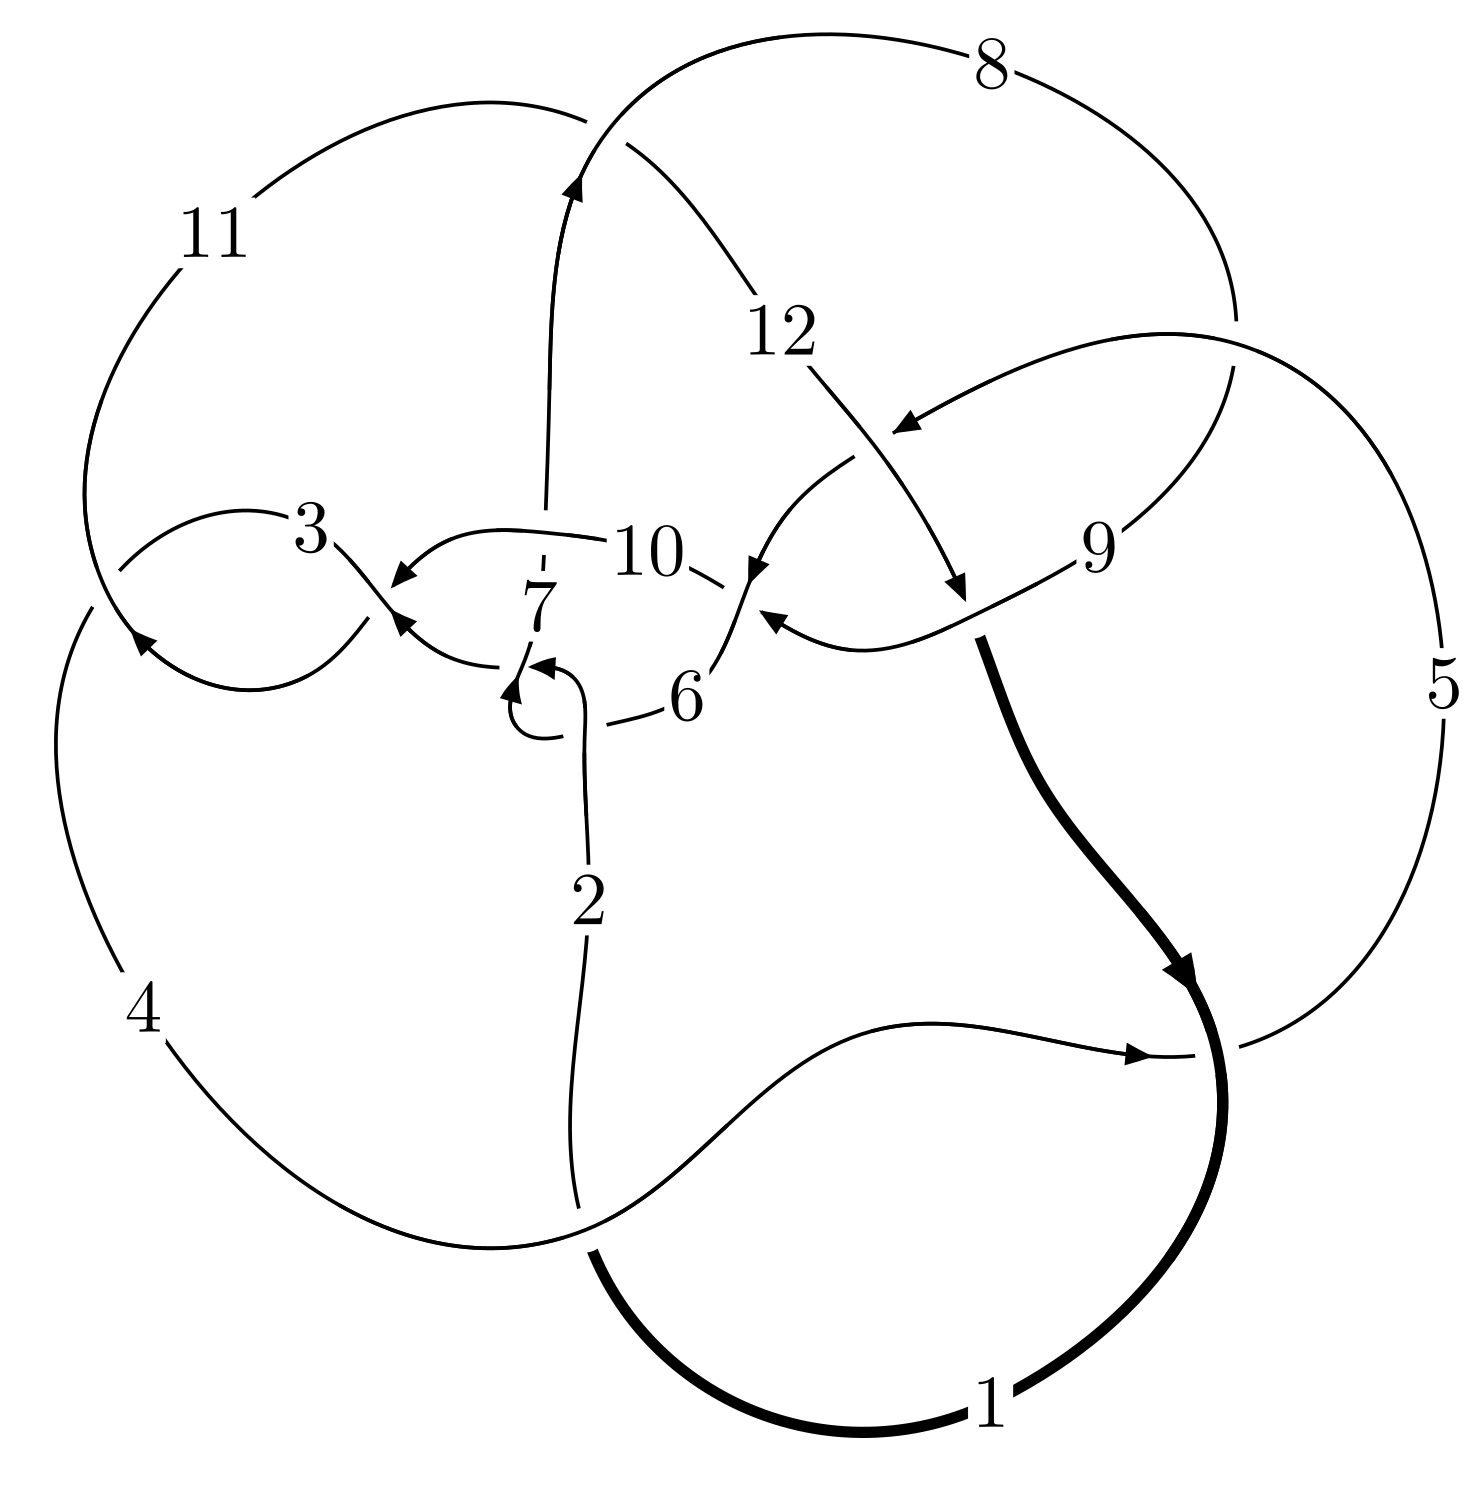
\includegraphics[width=112pt]{../../../GIT/diagram.site/Diagrams/png/1910_12a_1109.png}\\
\ \ \ A knot diagram\footnotemark}&
\allowdisplaybreaks
\textbf{Linearized knot diagam} \\
\cline{2-2}
 &
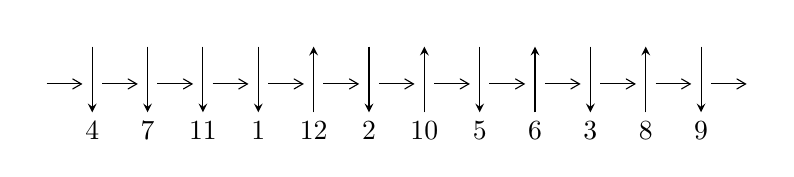
\begin{tikzpicture}[x=20pt, y=17pt]
	% nodes
	\node (C0) at (0, 0) {};
	\node (C1) at (1, 0) {};
	\node (C1U) at (1, +1) {};
	\node (C1D) at (1, -1) {4};

	\node (C2) at (2, 0) {};
	\node (C2U) at (2, +1) {};
	\node (C2D) at (2, -1) {7};

	\node (C3) at (3, 0) {};
	\node (C3U) at (3, +1) {};
	\node (C3D) at (3, -1) {11};

	\node (C4) at (4, 0) {};
	\node (C4U) at (4, +1) {};
	\node (C4D) at (4, -1) {1};

	\node (C5) at (5, 0) {};
	\node (C5U) at (5, +1) {};
	\node (C5D) at (5, -1) {12};

	\node (C6) at (6, 0) {};
	\node (C6U) at (6, +1) {};
	\node (C6D) at (6, -1) {2};

	\node (C7) at (7, 0) {};
	\node (C7U) at (7, +1) {};
	\node (C7D) at (7, -1) {10};

	\node (C8) at (8, 0) {};
	\node (C8U) at (8, +1) {};
	\node (C8D) at (8, -1) {5};

	\node (C9) at (9, 0) {};
	\node (C9U) at (9, +1) {};
	\node (C9D) at (9, -1) {6};

	\node (C10) at (10, 0) {};
	\node (C10U) at (10, +1) {};
	\node (C10D) at (10, -1) {3};

	\node (C11) at (11, 0) {};
	\node (C11U) at (11, +1) {};
	\node (C11D) at (11, -1) {8};

	\node (C12) at (12, 0) {};
	\node (C12U) at (12, +1) {};
	\node (C12D) at (12, -1) {9};
	\node (C13) at (13, 0) {};

	% arrows
	\draw[->,>={angle 60}]
	(C0) edge (C1) (C1) edge (C2) (C2) edge (C3) (C3) edge (C4) (C4) edge (C5) (C5) edge (C6) (C6) edge (C7) (C7) edge (C8) (C8) edge (C9) (C9) edge (C10) (C10) edge (C11) (C11) edge (C12) (C12) edge (C13) ;	\draw[->,>=stealth]
	(C1U) edge (C1D) (C2U) edge (C2D) (C3U) edge (C3D) (C4U) edge (C4D) (C5D) edge (C5U) (C6U) edge (C6D) (C7D) edge (C7U) (C8U) edge (C8D) (C9D) edge (C9U) (C10U) edge (C10D) (C11D) edge (C11U) (C12U) edge (C12D) ;
	\end{tikzpicture} \\
\hhline{~~} \\& 
\textbf{Solving Sequence} \\ \cline{2-2} 
 &
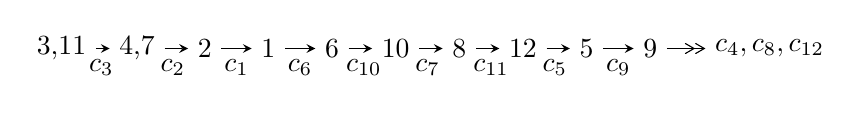
\begin{tikzpicture}[x=23pt, y=7pt]
	% node
	\node (A0) at (-1/8, 0) {3,11};
	\node (A1) at (17/16, 0) {4,7};
	\node (A2) at (17/8, 0) {2};
	\node (A3) at (25/8, 0) {1};
	\node (A4) at (33/8, 0) {6};
	\node (A5) at (41/8, 0) {10};
	\node (A6) at (49/8, 0) {8};
	\node (A7) at (57/8, 0) {12};
	\node (A8) at (65/8, 0) {5};
	\node (A9) at (73/8, 0) {9};
	\node (C1) at (1/2, -1) {$c_{3}$};
	\node (C2) at (13/8, -1) {$c_{2}$};
	\node (C3) at (21/8, -1) {$c_{1}$};
	\node (C4) at (29/8, -1) {$c_{6}$};
	\node (C5) at (37/8, -1) {$c_{10}$};
	\node (C6) at (45/8, -1) {$c_{7}$};
	\node (C7) at (53/8, -1) {$c_{11}$};
	\node (C8) at (61/8, -1) {$c_{5}$};
	\node (C9) at (69/8, -1) {$c_{9}$};
	\node (A10) at (11, 0) {$c_{4},c_{8},c_{12}$};

	% edge
	\draw[->,>=stealth]	
	(A0) edge (A1) (A1) edge (A2) (A2) edge (A3) (A3) edge (A4) (A4) edge (A5) (A5) edge (A6) (A6) edge (A7) (A7) edge (A8) (A8) edge (A9) ;
	\draw[->>,>={angle 60}]	
	(A9) edge (A10);
\end{tikzpicture} \\ 

\end{tabular} \\

\footnotetext{
The image of knot diagram is generated by the software ``\textbf{Draw programme}" developed by Andrew Bartholomew(\url{http://www.layer8.co.uk/maths/draw/index.htm\#Running-draw}), where we modified some parts for our purpose(\url{https://github.com/CATsTAILs/LinksPainter}).
}\phantom \\ \newline 
\centering \textbf{Ideals for irreducible components\footnotemark of $X_{\text{par}}$} 
 
\begin{align*}
I^u_{1}&=\langle 
b+u,\;-5.51351\times10^{20} u^{32}-1.00345\times10^{20} u^{31}+\cdots+4.96956\times10^{20} a-2.61633\times10^{21},\\
\phantom{I^u_{1}}&\phantom{= \langle  }u^{33}-13 u^{31}+\cdots+5 u-1\rangle \\
I^u_{2}&=\langle 
-2.42889\times10^{666} u^{125}+3.63484\times10^{665} u^{124}+\cdots+2.10762\times10^{666} b-2.25797\times10^{671},\\
\phantom{I^u_{2}}&\phantom{= \langle  }-4.35538\times10^{671} u^{125}+2.72760\times10^{670} u^{124}+\cdots+1.67305\times10^{671} a-3.95770\times10^{676},\\
\phantom{I^u_{2}}&\phantom{= \langle  }u^{126}- u^{125}+\cdots+445179 u-79381\rangle \\
I^u_{3}&=\langle 
b+u,\;188 u^{17}-64 u^{16}+\cdots+75 a-796,\;u^{18}-7 u^{16}+\cdots-3 u-1\rangle \\
I^u_{4}&=\langle 
14246904 u^{17}-7271564 u^{16}+\cdots+21285647 b-49419894,\\
\phantom{I^u_{4}}&\phantom{= \langle  }34578671 u^{17}+14037986 u^{16}+\cdots+21285647 a+25444982,\;u^{18}-8 u^{16}+\cdots- u-1\rangle \\
\\
\end{align*}
\raggedright * 4 irreducible components of $\dim_{\mathbb{C}}=0$, with total 195 representations.\\
\footnotetext{All coefficients of polynomials are rational numbers. But the coefficients are sometimes approximated in decimal forms when there is not enough margin.}
\newpage
\renewcommand{\arraystretch}{1}
\centering \section*{I. $I^u_{1}= \langle b+u,\;-5.51\times10^{20} u^{32}-1.00\times10^{20} u^{31}+\cdots+4.97\times10^{20} a-2.62\times10^{21},\;u^{33}-13 u^{31}+\cdots+5 u-1 \rangle$}
\flushleft \textbf{(i) Arc colorings}\\
\begin{tabular}{m{7pt} m{180pt} m{7pt} m{180pt} }
\flushright $a_{3}=$&$\begin{pmatrix}1\\0\end{pmatrix}$ \\
\flushright $a_{11}=$&$\begin{pmatrix}0\\u\end{pmatrix}$ \\
\flushright $a_{4}=$&$\begin{pmatrix}1\\u^2\end{pmatrix}$ \\
\flushright $a_{7}=$&$\begin{pmatrix}1.10946 u^{32}+0.201920 u^{31}+\cdots-4.37332 u+5.26470\\- u\end{pmatrix}$ \\
\flushright $a_{2}=$&$\begin{pmatrix}0.201920 u^{32}+0.164749 u^{31}+\cdots-0.282581 u+2.10946\\- u^2\end{pmatrix}$ \\
\flushright $a_{1}=$&$\begin{pmatrix}0.255700 u^{32}+0.133298 u^{31}+\cdots+0.339246 u+1.94471\\0.114568 u^{32}+0.000982119 u^{31}+\cdots+0.211036 u-0.0314510\end{pmatrix}$ \\
\flushright $a_{6}=$&$\begin{pmatrix}0.944707 u^{32}+0.255700 u^{31}+\cdots-5.47318 u+5.06278\\u^3- u\end{pmatrix}$ \\
\flushright $a_{10}=$&$\begin{pmatrix}u\\u\end{pmatrix}$ \\
\flushright $a_{8}=$&$\begin{pmatrix}0.944707 u^{32}+0.255700 u^{31}+\cdots-4.47318 u+5.06278\\-0.164749 u^{32}+0.0537806 u^{31}+\cdots-1.09986 u-0.201920\end{pmatrix}$ \\
\flushright $a_{12}=$&$\begin{pmatrix}1.10599 u^{32}+0.285758 u^{31}+\cdots-2.11902 u+5.03823\\-0.0881370 u^{32}-0.0855275 u^{31}+\cdots+1.99609 u-0.626985\end{pmatrix}$ \\
\flushright $a_{5}=$&$\begin{pmatrix}-0.185676 u^{32}+0.000949724 u^{31}+\cdots+0.432526 u+0.710133\\0.208808 u^{32}-0.0230167 u^{31}+\cdots-0.144418 u+0.0874475\end{pmatrix}$ \\
\flushright $a_{9}=$&$\begin{pmatrix}-1.00512 u^{32}-0.235683 u^{31}+\cdots+2.95587 u-4.84331\\0.100865 u^{32}+0.0500742 u^{31}+\cdots+0.836846 u+0.194913\end{pmatrix}$\\&\end{tabular}
\flushleft \textbf{(ii) Obstruction class $= -1$}\\~\\
\flushleft \textbf{(iii) Cusp Shapes $= \frac{11742058737997963033618}{4472604412221102382125} u^{32}+\frac{4842323161366125049279}{4472604412221102382125} u^{31}+\cdots-\frac{89973330678246945712378}{4472604412221102382125} u+\frac{44302109184650100143056}{4472604412221102382125}$}\\~\\
\newpage\renewcommand{\arraystretch}{1}
\flushleft \textbf{(iv) u-Polynomials at the component}\newline \\
\begin{tabular}{m{50pt}|m{274pt}}
Crossings & \hspace{64pt}u-Polynomials at each crossing \\
\hline $$\begin{aligned}c_{1},c_{4}\end{aligned}$$&$\begin{aligned}
&3(3 u^{33}-68 u^{32}+\cdots+6656 u-512)
\end{aligned}$\\
\hline $$\begin{aligned}c_{2},c_{3},c_{6}\\c_{10}\end{aligned}$$&$\begin{aligned}
&u^{33}-13 u^{31}+\cdots+5 u-1
\end{aligned}$\\
\hline $$\begin{aligned}c_{5}\end{aligned}$$&$\begin{aligned}
&3(3 u^{33}-83 u^{32}+\cdots+416 u-64)
\end{aligned}$\\
\hline $$\begin{aligned}c_{7}\end{aligned}$$&$\begin{aligned}
&3(3 u^{33}+83 u^{32}+\cdots+19456 u+4096)
\end{aligned}$\\
\hline $$\begin{aligned}c_{8},c_{12}\end{aligned}$$&$\begin{aligned}
&u^{33}+u^{32}+\cdots+8 u+3
\end{aligned}$\\
\hline $$\begin{aligned}c_{9},c_{11}\end{aligned}$$&$\begin{aligned}
&u^{33}+u^{32}+\cdots+8 u-29
\end{aligned}$\\
\hline
\end{tabular}\\~\\
\newpage\renewcommand{\arraystretch}{1}
\flushleft \textbf{(v) Riley Polynomials at the component}\newline \\
\begin{tabular}{m{50pt}|m{274pt}}
Crossings & \hspace{64pt}Riley Polynomials at each crossing \\
\hline $$\begin{aligned}c_{1},c_{4}\end{aligned}$$&$\begin{aligned}
&9(9 y^{33}+26 y^{32}+\cdots+1.25829\times10^{7} y-262144)
\end{aligned}$\\
\hline $$\begin{aligned}c_{2},c_{3},c_{6}\\c_{10}\end{aligned}$$&$\begin{aligned}
&y^{33}-26 y^{32}+\cdots+7 y-1
\end{aligned}$\\
\hline $$\begin{aligned}c_{5}\end{aligned}$$&$\begin{aligned}
&9(9 y^{33}-181 y^{32}+\cdots-89088 y-4096)
\end{aligned}$\\
\hline $$\begin{aligned}c_{7}\end{aligned}$$&$\begin{aligned}
&9(9 y^{33}-187 y^{32}+\cdots+4.39353\times10^{8} y-1.67772\times10^{7})
\end{aligned}$\\
\hline $$\begin{aligned}c_{8},c_{12}\end{aligned}$$&$\begin{aligned}
&y^{33}+5 y^{32}+\cdots+220 y-9
\end{aligned}$\\
\hline $$\begin{aligned}c_{9},c_{11}\end{aligned}$$&$\begin{aligned}
&y^{33}-17 y^{32}+\cdots+10620 y-841
\end{aligned}$\\
\hline
\end{tabular}\\~\\
\newpage\flushleft \textbf{(vi) Complex Volumes and Cusp Shapes}
$$\begin{array}{c|c|c}  
\text{Solutions to }I^u_{1}& \I (\text{vol} + \sqrt{-1}CS) & \text{Cusp shape}\\
 \hline 
\begin{aligned}
u &= -0.988042\phantom{ +0.000000I} \\
a &= \phantom{-}5.69224\phantom{ +0.000000I} \\
b &= \phantom{-}0.988042\phantom{ +0.000000I}\end{aligned}
 & \phantom{-}0.389613\phantom{ +0.000000I} & -30.4490\phantom{ +0.000000I} \\ \hline\begin{aligned}
u &= -0.738304 + 0.649893 I \\
a &= \phantom{-}0.098544 + 0.662865 I \\
b &= \phantom{-}0.738304 - 0.649893 I\end{aligned}
 & \phantom{-}5.00094 - 3.09470 I & \phantom{-}0.408039 + 0.525523 I \\ \hline\begin{aligned}
u &= -0.738304 - 0.649893 I \\
a &= \phantom{-}0.098544 - 0.662865 I \\
b &= \phantom{-}0.738304 + 0.649893 I\end{aligned}
 & \phantom{-}5.00094 + 3.09470 I & \phantom{-}0.408039 - 0.525523 I \\ \hline\begin{aligned}
u &= \phantom{-}1.002920 + 0.182034 I \\
a &= -3.32561 - 0.46867 I \\
b &= -1.002920 - 0.182034 I\end{aligned}
 & \phantom{-}3.90996 - 10.24170 I & -4.98610 + 7.85593 I \\ \hline\begin{aligned}
u &= \phantom{-}1.002920 - 0.182034 I \\
a &= -3.32561 + 0.46867 I \\
b &= -1.002920 + 0.182034 I\end{aligned}
 & \phantom{-}3.90996 + 10.24170 I & -4.98610 - 7.85593 I \\ \hline\begin{aligned}
u &= \phantom{-}0.354707 + 0.838712 I \\
a &= -0.949703 + 0.077776 I \\
b &= -0.354707 - 0.838712 I\end{aligned}
 & \phantom{-}7.49019 + 0.59025 I & \phantom{-}6.83489 - 0.22860 I \\ \hline\begin{aligned}
u &= \phantom{-}0.354707 - 0.838712 I \\
a &= -0.949703 - 0.077776 I \\
b &= -0.354707 + 0.838712 I\end{aligned}
 & \phantom{-}7.49019 - 0.59025 I & \phantom{-}6.83489 + 0.22860 I \\ \hline\begin{aligned}
u &= -0.305032 + 0.831776 I \\
a &= \phantom{-}1.269700 + 0.160717 I \\
b &= \phantom{-}0.305032 - 0.831776 I\end{aligned}
 & \phantom{-}8.03993 - 9.04618 I & \phantom{-}2.12985 + 4.01485 I \\ \hline\begin{aligned}
u &= -0.305032 - 0.831776 I \\
a &= \phantom{-}1.269700 - 0.160717 I \\
b &= \phantom{-}0.305032 + 0.831776 I\end{aligned}
 & \phantom{-}8.03993 + 9.04618 I & \phantom{-}2.12985 - 4.01485 I \\ \hline\begin{aligned}
u &= -0.015597 + 0.759933 I \\
a &= -0.276956 + 0.620225 I \\
b &= \phantom{-}0.015597 - 0.759933 I\end{aligned}
 & \phantom{-}3.45596 + 4.59127 I & \phantom{-}2.60162 - 5.91506 I\\
 \hline 
 \end{array}$$\newpage$$\begin{array}{c|c|c}  
\text{Solutions to }I^u_{1}& \I (\text{vol} + \sqrt{-1}CS) & \text{Cusp shape}\\
 \hline 
\begin{aligned}
u &= -0.015597 - 0.759933 I \\
a &= -0.276956 - 0.620225 I \\
b &= \phantom{-}0.015597 + 0.759933 I\end{aligned}
 & \phantom{-}3.45596 - 4.59127 I & \phantom{-}2.60162 + 5.91506 I \\ \hline\begin{aligned}
u &= \phantom{-}1.185980 + 0.380637 I \\
a &= -1.77450 + 1.34872 I \\
b &= -1.185980 - 0.380637 I\end{aligned}
 & -3.31674 - 2.54544 I & -5.71023 + 1.18268 I \\ \hline\begin{aligned}
u &= \phantom{-}1.185980 - 0.380637 I \\
a &= -1.77450 - 1.34872 I \\
b &= -1.185980 + 0.380637 I\end{aligned}
 & -3.31674 + 2.54544 I & -5.71023 - 1.18268 I \\ \hline\begin{aligned}
u &= -0.710776\phantom{ +0.000000I} \\
a &= \phantom{-}0.439454\phantom{ +0.000000I} \\
b &= \phantom{-}0.710776\phantom{ +0.000000I}\end{aligned}
 & -1.12251\phantom{ +0.000000I} & -6.37110\phantom{ +0.000000I} \\ \hline\begin{aligned}
u &= \phantom{-}0.505026 + 0.474040 I \\
a &= \phantom{-}0.398174 - 0.651892 I \\
b &= -0.505026 - 0.474040 I\end{aligned}
 & \phantom{-}3.18560 - 1.37010 I & -2.46667 + 3.82678 I \\ \hline\begin{aligned}
u &= \phantom{-}0.505026 - 0.474040 I \\
a &= \phantom{-}0.398174 + 0.651892 I \\
b &= -0.505026 + 0.474040 I\end{aligned}
 & \phantom{-}3.18560 + 1.37010 I & -2.46667 - 3.82678 I \\ \hline\begin{aligned}
u &= -1.291930 + 0.311595 I \\
a &= \phantom{-}1.46041 + 0.85218 I \\
b &= \phantom{-}1.291930 - 0.311595 I\end{aligned}
 & -7.56174 - 0.61747 I & -11.13526 + 2.09611 I \\ \hline\begin{aligned}
u &= -1.291930 - 0.311595 I \\
a &= \phantom{-}1.46041 - 0.85218 I \\
b &= \phantom{-}1.291930 + 0.311595 I\end{aligned}
 & -7.56174 + 0.61747 I & -11.13526 - 2.09611 I \\ \hline\begin{aligned}
u &= \phantom{-}1.324490 + 0.182144 I \\
a &= -1.75789 + 0.39816 I \\
b &= -1.324490 - 0.182144 I\end{aligned}
 & -6.90993 - 0.81575 I & -13.00695 - 0.18547 I \\ \hline\begin{aligned}
u &= \phantom{-}1.324490 - 0.182144 I \\
a &= -1.75789 - 0.39816 I \\
b &= -1.324490 + 0.182144 I\end{aligned}
 & -6.90993 + 0.81575 I & -13.00695 + 0.18547 I\\
 \hline 
 \end{array}$$\newpage$$\begin{array}{c|c|c}  
\text{Solutions to }I^u_{1}& \I (\text{vol} + \sqrt{-1}CS) & \text{Cusp shape}\\
 \hline 
\begin{aligned}
u &= -1.32813 + 0.48664 I \\
a &= \phantom{-}1.67278 + 0.89038 I \\
b &= \phantom{-}1.32813 - 0.48664 I\end{aligned}
 & -4.6785 + 13.5930 I & -6.98219 - 10.34778 I \\ \hline\begin{aligned}
u &= -1.32813 - 0.48664 I \\
a &= \phantom{-}1.67278 - 0.89038 I \\
b &= \phantom{-}1.32813 + 0.48664 I\end{aligned}
 & -4.6785 - 13.5930 I & -6.98219 + 10.34778 I \\ \hline\begin{aligned}
u &= \phantom{-}1.38591 + 0.41952 I \\
a &= -1.65623 + 0.48889 I \\
b &= -1.38591 - 0.41952 I\end{aligned}
 & -8.37796 - 5.05371 I & -12.03006 + 2.98505 I \\ \hline\begin{aligned}
u &= \phantom{-}1.38591 - 0.41952 I \\
a &= -1.65623 - 0.48889 I \\
b &= -1.38591 + 0.41952 I\end{aligned}
 & -8.37796 + 5.05371 I & -12.03006 - 2.98505 I \\ \hline\begin{aligned}
u &= -1.42702 + 0.32964 I \\
a &= \phantom{-}1.67206 + 0.08112 I \\
b &= \phantom{-}1.42702 - 0.32964 I\end{aligned}
 & -3.55978 + 5.14975 I & -8.65604 - 3.93341 I \\ \hline\begin{aligned}
u &= -1.42702 - 0.32964 I \\
a &= \phantom{-}1.67206 - 0.08112 I \\
b &= \phantom{-}1.42702 + 0.32964 I\end{aligned}
 & -3.55978 - 5.14975 I & -8.65604 + 3.93341 I \\ \hline\begin{aligned}
u &= -1.38771 + 0.56081 I \\
a &= \phantom{-}1.76185 + 0.49558 I \\
b &= \phantom{-}1.38771 - 0.56081 I\end{aligned}
 & \phantom{-}0.76112 + 11.54690 I & \phantom{-0.000000 } 0. - 8.50232 I \\ \hline\begin{aligned}
u &= -1.38771 - 0.56081 I \\
a &= \phantom{-}1.76185 - 0.49558 I \\
b &= \phantom{-}1.38771 + 0.56081 I\end{aligned}
 & \phantom{-}0.76112 - 11.54690 I & \phantom{-0.000000 -}0. + 8.50232 I \\ \hline\begin{aligned}
u &= \phantom{-}1.41446 + 0.61544 I \\
a &= -1.63169 + 0.52570 I \\
b &= -1.41446 - 0.61544 I\end{aligned}
 & \phantom{-}0.9133 - 20.5211 I & \phantom{-0.000000 -}0. + 10.13871 I \\ \hline\begin{aligned}
u &= \phantom{-}1.41446 - 0.61544 I \\
a &= -1.63169 - 0.52570 I \\
b &= -1.41446 + 0.61544 I\end{aligned}
 & \phantom{-}0.9133 + 20.5211 I & \phantom{-0.000000 } 0. - 10.13871 I\\
 \hline 
 \end{array}$$\newpage$$\begin{array}{c|c|c}  
\text{Solutions to }I^u_{1}& \I (\text{vol} + \sqrt{-1}CS) & \text{Cusp shape}\\
 \hline 
\begin{aligned}
u &= \phantom{-}0.045978 + 0.364709 I \\
a &= \phantom{-}1.56117 - 0.41807 I \\
b &= -0.045978 - 0.364709 I\end{aligned}
 & -0.09428 + 1.57059 I & -1.17905 - 4.36541 I \\ \hline\begin{aligned}
u &= \phantom{-}0.045978 - 0.364709 I \\
a &= \phantom{-}1.56117 + 0.41807 I \\
b &= -0.045978 + 0.364709 I\end{aligned}
 & -0.09428 - 1.57059 I & -1.17905 + 4.36541 I \\ \hline\begin{aligned}
u &= \phantom{-}0.247344\phantom{ +0.000000I} \\
a &= \phantom{-}5.15743\phantom{ +0.000000I} \\
b &= -0.247344\phantom{ +0.000000I}\end{aligned}
 & \phantom{-}2.57187\phantom{ +0.000000I} & \phantom{-}8.03110\phantom{ +0.000000I}\\
 \hline 
 \end{array}$$\newpage\newpage\renewcommand{\arraystretch}{1}
\centering \section*{II. $I^u_{2}= \langle -2.43\times10^{666} u^{125}+3.63\times10^{665} u^{124}+\cdots+2.11\times10^{666} b-2.26\times10^{671},\;-4.36\times10^{671} u^{125}+2.73\times10^{670} u^{124}+\cdots+1.67\times10^{671} a-3.96\times10^{676},\;u^{126}- u^{125}+\cdots+445179 u-79381 \rangle$}
\flushleft \textbf{(i) Arc colorings}\\
\begin{tabular}{m{7pt} m{180pt} m{7pt} m{180pt} }
\flushright $a_{3}=$&$\begin{pmatrix}1\\0\end{pmatrix}$ \\
\flushright $a_{11}=$&$\begin{pmatrix}0\\u\end{pmatrix}$ \\
\flushright $a_{4}=$&$\begin{pmatrix}1\\u^2\end{pmatrix}$ \\
\flushright $a_{7}=$&$\begin{pmatrix}2.60326 u^{125}-0.163032 u^{124}+\cdots-1.07321\times10^{6} u+236556.\\1.15243 u^{125}-0.172462 u^{124}+\cdots-476233. u+107134.\end{pmatrix}$ \\
\flushright $a_{2}=$&$\begin{pmatrix}3.60912 u^{125}-0.273875 u^{124}+\cdots-1.49893\times10^{6} u+331671.\\1.98933 u^{125}-0.303058 u^{124}+\cdots-845433. u+190405.\end{pmatrix}$ \\
\flushright $a_{1}=$&$\begin{pmatrix}2.75193 u^{125}-0.382917 u^{124}+\cdots-1.14608\times10^{6} u+257320.\\1.12658 u^{125}-0.399171 u^{124}+\cdots-483331. u+113705.\end{pmatrix}$ \\
\flushright $a_{6}=$&$\begin{pmatrix}-0.0908361 u^{125}+0.138689 u^{124}+\cdots+91584.7 u-23023.8\\0.960737 u^{125}+0.0952325 u^{124}+\cdots-288454. u+60008.7\end{pmatrix}$ \\
\flushright $a_{10}=$&$\begin{pmatrix}u\\u\end{pmatrix}$ \\
\flushright $a_{8}=$&$\begin{pmatrix}1.32650 u^{125}-0.178769 u^{124}+\cdots-538299. u+120639.\\-0.124328 u^{125}-0.188199 u^{124}+\cdots+58675.8 u-8782.80\end{pmatrix}$ \\
\flushright $a_{12}=$&$\begin{pmatrix}-2.02791 u^{125}+0.315409 u^{124}+\cdots+824363. u-185723.\\-0.0189666 u^{125}+0.105342 u^{124}+\cdots+105576. u-26189.8\end{pmatrix}$ \\
\flushright $a_{5}=$&$\begin{pmatrix}7.08729 u^{125}-0.363708 u^{124}+\cdots-2.76880\times10^{6} u+608251.\\5.64107 u^{125}+0.170762 u^{124}+\cdots-2.39045\times10^{6} u+516688.\end{pmatrix}$ \\
\flushright $a_{9}=$&$\begin{pmatrix}13.5383 u^{125}-1.09910 u^{124}+\cdots-5.28559\times10^{6} u+1.16915\times10^{6}\\14.3116 u^{125}-1.33426 u^{124}+\cdots-5.61938\times10^{6} u+1.24685\times10^{6}\end{pmatrix}$\\&\end{tabular}
\flushleft \textbf{(ii) Obstruction class $= -1$}\\~\\
\flushleft \textbf{(iii) Cusp Shapes $= 13.1438 u^{125}-2.17406 u^{124}+\cdots-4.54071\times10^{6} u+1.02447\times10^{6}$}\\~\\
\newpage\renewcommand{\arraystretch}{1}
\flushleft \textbf{(iv) u-Polynomials at the component}\newline \\
\begin{tabular}{m{50pt}|m{274pt}}
Crossings & \hspace{64pt}u-Polynomials at each crossing \\
\hline $$\begin{aligned}c_{1},c_{4}\end{aligned}$$&$\begin{aligned}
&(u^{63}+11 u^{62}+\cdots+159 u-1)^{2}
\end{aligned}$\\
\hline $$\begin{aligned}c_{2},c_{3},c_{6}\\c_{10}\end{aligned}$$&$\begin{aligned}
&u^{126}- u^{125}+\cdots+445179 u-79381
\end{aligned}$\\
\hline $$\begin{aligned}c_{5}\end{aligned}$$&$\begin{aligned}
&(u^{63}+16 u^{62}+\cdots+5 u+1)^{2}
\end{aligned}$\\
\hline $$\begin{aligned}c_{7}\end{aligned}$$&$\begin{aligned}
&(u^{63}-14 u^{62}+\cdots-694 u+39)^{2}
\end{aligned}$\\
\hline $$\begin{aligned}c_{8},c_{12}\end{aligned}$$&$\begin{aligned}
&u^{126}+8 u^{125}+\cdots-23405 u-2473
\end{aligned}$\\
\hline $$\begin{aligned}c_{9},c_{11}\end{aligned}$$&$\begin{aligned}
&u^{126}-2 u^{125}+\cdots-81829844 u-30650633
\end{aligned}$\\
\hline
\end{tabular}\\~\\
\newpage\renewcommand{\arraystretch}{1}
\flushleft \textbf{(v) Riley Polynomials at the component}\newline \\
\begin{tabular}{m{50pt}|m{274pt}}
Crossings & \hspace{64pt}Riley Polynomials at each crossing \\
\hline $$\begin{aligned}c_{1},c_{4}\end{aligned}$$&$\begin{aligned}
&(y^{63}+35 y^{62}+\cdots+29501 y-1)^{2}
\end{aligned}$\\
\hline $$\begin{aligned}c_{2},c_{3},c_{6}\\c_{10}\end{aligned}$$&$\begin{aligned}
&y^{126}-85 y^{125}+\cdots-14924889155 y+6301343161
\end{aligned}$\\
\hline $$\begin{aligned}c_{5}\end{aligned}$$&$\begin{aligned}
&(y^{63}-26 y^{62}+\cdots+47 y-1)^{2}
\end{aligned}$\\
\hline $$\begin{aligned}c_{7}\end{aligned}$$&$\begin{aligned}
&(y^{63}-104 y^{61}+\cdots+27910 y-1521)^{2}
\end{aligned}$\\
\hline $$\begin{aligned}c_{8},c_{12}\end{aligned}$$&$\begin{aligned}
&y^{126}+32 y^{125}+\cdots-362675137 y+6115729
\end{aligned}$\\
\hline $$\begin{aligned}c_{9},c_{11}\end{aligned}$$&$\begin{aligned}
&y^{126}-58 y^{125}+\cdots-22519621465061486 y+939461303300689
\end{aligned}$\\
\hline
\end{tabular}\\~\\
\newpage\flushleft \textbf{(vi) Complex Volumes and Cusp Shapes}
$$\begin{array}{c|c|c}  
\text{Solutions to }I^u_{2}& \I (\text{vol} + \sqrt{-1}CS) & \text{Cusp shape}\\
 \hline 
\begin{aligned}
u &= \phantom{-}0.231017 + 0.974102 I \\
a &= -0.161333 + 0.201744 I \\
b &= -1.223380 + 0.555574 I\end{aligned}
 & \phantom{-}2.80266 + 5.31618 I & \phantom{-0.000000 } 0 \\ \hline\begin{aligned}
u &= \phantom{-}0.231017 - 0.974102 I \\
a &= -0.161333 - 0.201744 I \\
b &= -1.223380 - 0.555574 I\end{aligned}
 & \phantom{-}2.80266 - 5.31618 I & \phantom{-0.000000 } 0 \\ \hline\begin{aligned}
u &= -0.726101 + 0.685259 I \\
a &= -0.712122 + 0.711786 I \\
b &= \phantom{-}0.475020 + 0.495981 I\end{aligned}
 & \phantom{-}4.00952 - 1.59909 I & \phantom{-0.000000 } 0 \\ \hline\begin{aligned}
u &= -0.726101 - 0.685259 I \\
a &= -0.712122 - 0.711786 I \\
b &= \phantom{-}0.475020 - 0.495981 I\end{aligned}
 & \phantom{-}4.00952 + 1.59909 I & \phantom{-0.000000 } 0 \\ \hline\begin{aligned}
u &= -0.945676 + 0.299992 I \\
a &= -2.86713 - 0.06400 I \\
b &= -0.958414 + 0.093245 I\end{aligned}
 & \phantom{-}2.80740 + 1.73216 I & \phantom{-0.000000 } 0 \\ \hline\begin{aligned}
u &= -0.945676 - 0.299992 I \\
a &= -2.86713 + 0.06400 I \\
b &= -0.958414 - 0.093245 I\end{aligned}
 & \phantom{-}2.80740 - 1.73216 I & \phantom{-0.000000 } 0 \\ \hline\begin{aligned}
u &= -1.01420\phantom{ +0.000000I} \\
a &= \phantom{-}3.19187\phantom{ +0.000000I} \\
b &= -0.739216\phantom{ +0.000000I}\end{aligned}
 & \phantom{-}0.282990\phantom{ +0.000000I} & \phantom{-0.000000 } 0 \\ \hline\begin{aligned}
u &= \phantom{-}0.186212 + 1.003630 I \\
a &= \phantom{-}1.198480 - 0.372593 I \\
b &= \phantom{-}0.560041 + 0.609185 I\end{aligned}
 & \phantom{-}6.05015 - 0.21785 I & \phantom{-0.000000 } 0 \\ \hline\begin{aligned}
u &= \phantom{-}0.186212 - 1.003630 I \\
a &= \phantom{-}1.198480 + 0.372593 I \\
b &= \phantom{-}0.560041 - 0.609185 I\end{aligned}
 & \phantom{-}6.05015 + 0.21785 I & \phantom{-0.000000 } 0 \\ \hline\begin{aligned}
u &= -0.968483 + 0.034921 I \\
a &= -2.52345 - 0.92440 I \\
b &= -1.382910 + 0.259862 I\end{aligned}
 & -1.14077 + 1.10990 I & \phantom{-0.000000 } 0\\
 \hline 
 \end{array}$$\newpage$$\begin{array}{c|c|c}  
\text{Solutions to }I^u_{2}& \I (\text{vol} + \sqrt{-1}CS) & \text{Cusp shape}\\
 \hline 
\begin{aligned}
u &= -0.968483 - 0.034921 I \\
a &= -2.52345 + 0.92440 I \\
b &= -1.382910 - 0.259862 I\end{aligned}
 & -1.14077 - 1.10990 I & \phantom{-0.000000 } 0 \\ \hline\begin{aligned}
u &= \phantom{-}0.933812 + 0.255135 I \\
a &= \phantom{-}0.515557 - 0.310399 I \\
b &= \phantom{-}0.022124 + 0.753927 I\end{aligned}
 & \phantom{-}0.72649 - 2.79094 I & \phantom{-0.000000 } 0 \\ \hline\begin{aligned}
u &= \phantom{-}0.933812 - 0.255135 I \\
a &= \phantom{-}0.515557 + 0.310399 I \\
b &= \phantom{-}0.022124 - 0.753927 I\end{aligned}
 & \phantom{-}0.72649 + 2.79094 I & \phantom{-0.000000 } 0 \\ \hline\begin{aligned}
u &= -0.383512 + 0.887504 I \\
a &= \phantom{-}0.0706374 + 0.0522425 I \\
b &= \phantom{-}1.153240 + 0.239311 I\end{aligned}
 & -0.93547 - 2.28826 I & \phantom{-0.000000 } 0 \\ \hline\begin{aligned}
u &= -0.383512 - 0.887504 I \\
a &= \phantom{-}0.0706374 - 0.0522425 I \\
b &= \phantom{-}1.153240 - 0.239311 I\end{aligned}
 & -0.93547 + 2.28826 I & \phantom{-0.000000 } 0 \\ \hline\begin{aligned}
u &= \phantom{-}0.958414 + 0.093245 I \\
a &= \phantom{-}2.90275 + 0.55187 I \\
b &= \phantom{-}0.945676 + 0.299992 I\end{aligned}
 & \phantom{-}2.80740 - 1.73216 I & \phantom{-0.000000 } 0 \\ \hline\begin{aligned}
u &= \phantom{-}0.958414 - 0.093245 I \\
a &= \phantom{-}2.90275 - 0.55187 I \\
b &= \phantom{-}0.945676 - 0.299992 I\end{aligned}
 & \phantom{-}2.80740 + 1.73216 I & \phantom{-0.000000 } 0 \\ \hline\begin{aligned}
u &= \phantom{-}1.048070 + 0.054620 I \\
a &= \phantom{-}2.44274 + 0.18348 I \\
b &= \phantom{-}2.02951 - 0.22269 I\end{aligned}
 & -0.91409 - 5.95546 I & \phantom{-0.000000 } 0 \\ \hline\begin{aligned}
u &= \phantom{-}1.048070 - 0.054620 I \\
a &= \phantom{-}2.44274 - 0.18348 I \\
b &= \phantom{-}2.02951 + 0.22269 I\end{aligned}
 & -0.91409 + 5.95546 I & \phantom{-0.000000 } 0 \\ \hline\begin{aligned}
u &= -1.056660 + 0.048917 I \\
a &= \phantom{-}1.47570 - 0.45195 I \\
b &= \phantom{-}1.228370 + 0.454325 I\end{aligned}
 & -1.71117 + 1.03772 I & \phantom{-0.000000 } 0\\
 \hline 
 \end{array}$$\newpage$$\begin{array}{c|c|c}  
\text{Solutions to }I^u_{2}& \I (\text{vol} + \sqrt{-1}CS) & \text{Cusp shape}\\
 \hline 
\begin{aligned}
u &= -1.056660 - 0.048917 I \\
a &= \phantom{-}1.47570 + 0.45195 I \\
b &= \phantom{-}1.228370 - 0.454325 I\end{aligned}
 & -1.71117 - 1.03772 I & \phantom{-0.000000 } 0 \\ \hline\begin{aligned}
u &= \phantom{-}0.092151 + 0.931553 I \\
a &= -0.434887 + 0.576532 I \\
b &= -1.222610 - 0.329948 I\end{aligned}
 & -0.38295 - 8.49628 I & \phantom{-0.000000 } 0 \\ \hline\begin{aligned}
u &= \phantom{-}0.092151 - 0.931553 I \\
a &= -0.434887 - 0.576532 I \\
b &= -1.222610 + 0.329948 I\end{aligned}
 & -0.38295 + 8.49628 I & \phantom{-0.000000 } 0 \\ \hline\begin{aligned}
u &= -0.990794 + 0.406870 I \\
a &= -0.565079 + 0.557528 I \\
b &= -0.23128 + 1.45237 I\end{aligned}
 & \phantom{-}4.70571 + 3.83850 I & \phantom{-0.000000 } 0 \\ \hline\begin{aligned}
u &= -0.990794 - 0.406870 I \\
a &= -0.565079 - 0.557528 I \\
b &= -0.23128 - 1.45237 I\end{aligned}
 & \phantom{-}4.70571 - 3.83850 I & \phantom{-0.000000 } 0 \\ \hline\begin{aligned}
u &= \phantom{-}0.926911 + 0.015610 I \\
a &= -2.55747 + 0.29813 I \\
b &= -1.95135 - 0.38954 I\end{aligned}
 & -0.31440 - 5.74271 I & \phantom{-0.000000 } 0 \\ \hline\begin{aligned}
u &= \phantom{-}0.926911 - 0.015610 I \\
a &= -2.55747 - 0.29813 I \\
b &= -1.95135 + 0.38954 I\end{aligned}
 & -0.31440 + 5.74271 I & \phantom{-0.000000 } 0 \\ \hline\begin{aligned}
u &= -0.969437 + 0.465037 I \\
a &= -0.589741 - 0.268638 I \\
b &= -0.700197 + 1.005260 I\end{aligned}
 & \phantom{-}3.18701 + 6.15547 I & \phantom{-0.000000 } 0 \\ \hline\begin{aligned}
u &= -0.969437 - 0.465037 I \\
a &= -0.589741 + 0.268638 I \\
b &= -0.700197 - 1.005260 I\end{aligned}
 & \phantom{-}3.18701 - 6.15547 I & \phantom{-0.000000 } 0 \\ \hline\begin{aligned}
u &= \phantom{-}0.960150 + 0.537279 I \\
a &= \phantom{-}0.527575 - 0.156061 I \\
b &= -0.036489 - 0.560410 I\end{aligned}
 & \phantom{-}3.14161 - 1.66960 I & \phantom{-0.000000 } 0\\
 \hline 
 \end{array}$$\newpage$$\begin{array}{c|c|c}  
\text{Solutions to }I^u_{2}& \I (\text{vol} + \sqrt{-1}CS) & \text{Cusp shape}\\
 \hline 
\begin{aligned}
u &= \phantom{-}0.960150 - 0.537279 I \\
a &= \phantom{-}0.527575 + 0.156061 I \\
b &= -0.036489 + 0.560410 I\end{aligned}
 & \phantom{-}3.14161 + 1.66960 I & \phantom{-0.000000 } 0 \\ \hline\begin{aligned}
u &= -0.873818 + 0.684520 I \\
a &= \phantom{-}0.524809 - 0.616571 I \\
b &= -0.721317 - 0.270053 I\end{aligned}
 & \phantom{-}4.68388 + 8.26965 I & \phantom{-0.000000 } 0 \\ \hline\begin{aligned}
u &= -0.873818 - 0.684520 I \\
a &= \phantom{-}0.524809 + 0.616571 I \\
b &= -0.721317 + 0.270053 I\end{aligned}
 & \phantom{-}4.68388 - 8.26965 I & \phantom{-0.000000 } 0 \\ \hline\begin{aligned}
u &= -1.107760 + 0.086604 I \\
a &= \phantom{-}0.187691 - 0.538217 I \\
b &= \phantom{-}0.244907 - 1.237800 I\end{aligned}
 & -3.04963 - 0.18332 I & \phantom{-0.000000 } 0 \\ \hline\begin{aligned}
u &= -1.107760 - 0.086604 I \\
a &= \phantom{-}0.187691 + 0.538217 I \\
b &= \phantom{-}0.244907 + 1.237800 I\end{aligned}
 & -3.04963 + 0.18332 I & \phantom{-0.000000 } 0 \\ \hline\begin{aligned}
u &= \phantom{-}0.882048 + 0.019394 I \\
a &= -0.0941606 + 0.0415742 I \\
b &= -0.705452 + 1.009270 I\end{aligned}
 & \phantom{-}3.20385 + 0.81417 I & \phantom{-0.000000 } 0 \\ \hline\begin{aligned}
u &= \phantom{-}0.882048 - 0.019394 I \\
a &= -0.0941606 - 0.0415742 I \\
b &= -0.705452 - 1.009270 I\end{aligned}
 & \phantom{-}3.20385 - 0.81417 I & \phantom{-0.000000 } 0 \\ \hline\begin{aligned}
u &= \phantom{-}1.151890 + 0.193176 I \\
a &= -0.244501 - 0.415125 I \\
b &= -0.051266 + 0.545218 I\end{aligned}
 & -3.26702 - 3.89641 I & \phantom{-0.000000 } 0 \\ \hline\begin{aligned}
u &= \phantom{-}1.151890 - 0.193176 I \\
a &= -0.244501 + 0.415125 I \\
b &= -0.051266 - 0.545218 I\end{aligned}
 & -3.26702 + 3.89641 I & \phantom{-0.000000 } 0 \\ \hline\begin{aligned}
u &= \phantom{-}1.073500 + 0.469067 I \\
a &= -0.321729 - 0.595620 I \\
b &= -0.061776 - 1.241670 I\end{aligned}
 & \phantom{-}5.25739 - 5.36322 I & \phantom{-0.000000 } 0\\
 \hline 
 \end{array}$$\newpage$$\begin{array}{c|c|c}  
\text{Solutions to }I^u_{2}& \I (\text{vol} + \sqrt{-1}CS) & \text{Cusp shape}\\
 \hline 
\begin{aligned}
u &= \phantom{-}1.073500 - 0.469067 I \\
a &= -0.321729 + 0.595620 I \\
b &= -0.061776 + 1.241670 I\end{aligned}
 & \phantom{-}5.25739 + 5.36322 I & \phantom{-0.000000 } 0 \\ \hline\begin{aligned}
u &= -0.560041 + 0.609185 I \\
a &= -1.49673 + 0.39580 I \\
b &= -0.186212 + 1.003630 I\end{aligned}
 & \phantom{-}6.05015 + 0.21785 I & \phantom{-0.000000 } 0 \\ \hline\begin{aligned}
u &= -0.560041 - 0.609185 I \\
a &= -1.49673 - 0.39580 I \\
b &= -0.186212 - 1.003630 I\end{aligned}
 & \phantom{-}6.05015 - 0.21785 I & \phantom{-0.000000 } 0 \\ \hline\begin{aligned}
u &= -1.172060 + 0.069673 I \\
a &= -1.81051 - 0.54262 I \\
b &= -1.53503 - 0.89173 I\end{aligned}
 & -3.42898 + 2.30117 I & \phantom{-0.000000 } 0 \\ \hline\begin{aligned}
u &= -1.172060 - 0.069673 I \\
a &= -1.81051 + 0.54262 I \\
b &= -1.53503 + 0.89173 I\end{aligned}
 & -3.42898 - 2.30117 I & \phantom{-0.000000 } 0 \\ \hline\begin{aligned}
u &= \phantom{-}1.161000 + 0.193168 I \\
a &= \phantom{-}2.20920 + 0.10935 I \\
b &= \phantom{-}1.50555 + 0.73851 I\end{aligned}
 & \phantom{-}0.20473 - 6.15765 I & \phantom{-0.000000 } 0 \\ \hline\begin{aligned}
u &= \phantom{-}1.161000 - 0.193168 I \\
a &= \phantom{-}2.20920 - 0.10935 I \\
b &= \phantom{-}1.50555 - 0.73851 I\end{aligned}
 & \phantom{-}0.20473 + 6.15765 I & \phantom{-0.000000 } 0 \\ \hline\begin{aligned}
u &= -1.153240 + 0.239311 I \\
a &= \phantom{-}0.0537071 + 0.0481322 I \\
b &= \phantom{-}0.383512 + 0.887504 I\end{aligned}
 & -0.93547 + 2.28826 I & \phantom{-0.000000 } 0 \\ \hline\begin{aligned}
u &= -1.153240 - 0.239311 I \\
a &= \phantom{-}0.0537071 - 0.0481322 I \\
b &= \phantom{-}0.383512 - 0.887504 I\end{aligned}
 & -0.93547 - 2.28826 I & \phantom{-0.000000 } 0 \\ \hline\begin{aligned}
u &= -1.146770 + 0.277757 I \\
a &= \phantom{-}0.697238 - 0.020965 I \\
b &= -0.058951 - 0.436078 I\end{aligned}
 & -0.131859 - 0.845720 I & \phantom{-0.000000 } 0\\
 \hline 
 \end{array}$$\newpage$$\begin{array}{c|c|c}  
\text{Solutions to }I^u_{2}& \I (\text{vol} + \sqrt{-1}CS) & \text{Cusp shape}\\
 \hline 
\begin{aligned}
u &= -1.146770 - 0.277757 I \\
a &= \phantom{-}0.697238 + 0.020965 I \\
b &= -0.058951 + 0.436078 I\end{aligned}
 & -0.131859 + 0.845720 I & \phantom{-0.000000 } 0 \\ \hline\begin{aligned}
u &= -1.160410 + 0.245312 I \\
a &= \phantom{-}2.07907 - 0.09023 I \\
b &= \phantom{-}1.69972 - 0.75102 I\end{aligned}
 & -0.24112 + 4.51482 I & \phantom{-0.000000 } 0 \\ \hline\begin{aligned}
u &= -1.160410 - 0.245312 I \\
a &= \phantom{-}2.07907 + 0.09023 I \\
b &= \phantom{-}1.69972 + 0.75102 I\end{aligned}
 & -0.24112 - 4.51482 I & \phantom{-0.000000 } 0 \\ \hline\begin{aligned}
u &= \phantom{-}0.700197 + 1.005260 I \\
a &= \phantom{-}0.334272 - 0.460166 I \\
b &= \phantom{-}0.969437 + 0.465037 I\end{aligned}
 & \phantom{-}3.18701 - 6.15547 I & \phantom{-0.000000 } 0 \\ \hline\begin{aligned}
u &= \phantom{-}0.700197 - 1.005260 I \\
a &= \phantom{-}0.334272 + 0.460166 I \\
b &= \phantom{-}0.969437 - 0.465037 I\end{aligned}
 & \phantom{-}3.18701 + 6.15547 I & \phantom{-0.000000 } 0 \\ \hline\begin{aligned}
u &= \phantom{-}0.721317 + 0.270053 I \\
a &= \phantom{-}0.364380 + 1.108540 I \\
b &= \phantom{-}0.873818 - 0.684520 I\end{aligned}
 & \phantom{-}4.68388 + 8.26965 I & \phantom{-0.000000 } 0 \\ \hline\begin{aligned}
u &= \phantom{-}0.721317 - 0.270053 I \\
a &= \phantom{-}0.364380 - 1.108540 I \\
b &= \phantom{-}0.873818 + 0.684520 I\end{aligned}
 & \phantom{-}4.68388 - 8.26965 I & \phantom{-0.000000 } 0 \\ \hline\begin{aligned}
u &= \phantom{-}0.705452 + 1.009270 I \\
a &= -0.0622091 + 0.0396078 I \\
b &= -0.882048 + 0.019394 I\end{aligned}
 & \phantom{-}3.20385 - 0.81417 I & \phantom{-0.000000 } 0 \\ \hline\begin{aligned}
u &= \phantom{-}0.705452 - 1.009270 I \\
a &= -0.0622091 - 0.0396078 I \\
b &= -0.882048 - 0.019394 I\end{aligned}
 & \phantom{-}3.20385 + 0.81417 I & \phantom{-0.000000 } 0 \\ \hline\begin{aligned}
u &= -0.759979\phantom{ +0.000000I} \\
a &= \phantom{-}0.415564\phantom{ +0.000000I} \\
b &= \phantom{-}0.631645\phantom{ +0.000000I}\end{aligned}
 & -1.12173\phantom{ +0.000000I} & \phantom{-0.000000 } 0\\
 \hline 
 \end{array}$$\newpage$$\begin{array}{c|c|c}  
\text{Solutions to }I^u_{2}& \I (\text{vol} + \sqrt{-1}CS) & \text{Cusp shape}\\
 \hline 
\begin{aligned}
u &= \phantom{-}0.061776 + 1.241670 I \\
a &= -0.637555 + 0.021425 I \\
b &= -1.073500 - 0.469067 I\end{aligned}
 & \phantom{-}5.25739 - 5.36322 I & \phantom{-0.000000 } 0 \\ \hline\begin{aligned}
u &= \phantom{-}0.061776 - 1.241670 I \\
a &= -0.637555 - 0.021425 I \\
b &= -1.073500 + 0.469067 I\end{aligned}
 & \phantom{-}5.25739 + 5.36322 I & \phantom{-0.000000 } 0 \\ \hline\begin{aligned}
u &= -0.022124 + 0.753927 I \\
a &= \phantom{-}0.188008 - 0.749126 I \\
b &= -0.933812 + 0.255135 I\end{aligned}
 & \phantom{-}0.72649 + 2.79094 I & \phantom{-0.000000 } 0 \\ \hline\begin{aligned}
u &= -0.022124 - 0.753927 I \\
a &= \phantom{-}0.188008 + 0.749126 I \\
b &= -0.933812 - 0.255135 I\end{aligned}
 & \phantom{-}0.72649 - 2.79094 I & \phantom{-0.000000 } 0 \\ \hline\begin{aligned}
u &= -1.169410 + 0.466173 I \\
a &= \phantom{-}0.215838 - 0.511817 I \\
b &= -0.023556 - 1.346520 I\end{aligned}
 & \phantom{-}5.3085 + 13.7961 I & \phantom{-0.000000 } 0 \\ \hline\begin{aligned}
u &= -1.169410 - 0.466173 I \\
a &= \phantom{-}0.215838 + 0.511817 I \\
b &= -0.023556 + 1.346520 I\end{aligned}
 & \phantom{-}5.3085 - 13.7961 I & \phantom{-0.000000 } 0 \\ \hline\begin{aligned}
u &= \phantom{-}0.739216\phantom{ +0.000000I} \\
a &= -4.37922\phantom{ +0.000000I} \\
b &= \phantom{-}1.01420\phantom{ +0.000000I}\end{aligned}
 & \phantom{-}0.282990\phantom{ +0.000000I} & \phantom{-0.000000 } 0 \\ \hline\begin{aligned}
u &= -0.244907 + 1.237800 I \\
a &= \phantom{-}0.500977 + 0.031194 I \\
b &= \phantom{-}1.107760 - 0.086604 I\end{aligned}
 & -3.04963 - 0.18332 I & \phantom{-0.000000 } 0 \\ \hline\begin{aligned}
u &= -0.244907 - 1.237800 I \\
a &= \phantom{-}0.500977 - 0.031194 I \\
b &= \phantom{-}1.107760 + 0.086604 I\end{aligned}
 & -3.04963 + 0.18332 I & \phantom{-0.000000 } 0 \\ \hline\begin{aligned}
u &= \phantom{-}1.222610 + 0.329948 I \\
a &= -0.512435 - 0.149610 I \\
b &= -0.092151 - 0.931553 I\end{aligned}
 & -0.38295 - 8.49628 I & \phantom{-0.000000 } 0\\
 \hline 
 \end{array}$$\newpage$$\begin{array}{c|c|c}  
\text{Solutions to }I^u_{2}& \I (\text{vol} + \sqrt{-1}CS) & \text{Cusp shape}\\
 \hline 
\begin{aligned}
u &= \phantom{-}1.222610 - 0.329948 I \\
a &= -0.512435 + 0.149610 I \\
b &= -0.092151 + 0.931553 I\end{aligned}
 & -0.38295 + 8.49628 I & \phantom{-0.000000 } 0 \\ \hline\begin{aligned}
u &= -1.151610 + 0.532353 I \\
a &= -1.39892 - 0.98201 I \\
b &= -1.315840 + 0.477195 I\end{aligned}
 & -3.35885 + 7.50906 I & \phantom{-0.000000 } 0 \\ \hline\begin{aligned}
u &= -1.151610 - 0.532353 I \\
a &= -1.39892 + 0.98201 I \\
b &= -1.315840 - 0.477195 I\end{aligned}
 & -3.35885 - 7.50906 I & \phantom{-0.000000 } 0 \\ \hline\begin{aligned}
u &= \phantom{-}1.017080 + 0.766078 I \\
a &= -0.223433 - 0.144013 I \\
b &= -0.203048 + 0.285531 I\end{aligned}
 & \phantom{-}3.11818 - 4.10927 I & \phantom{-0.000000 } 0 \\ \hline\begin{aligned}
u &= \phantom{-}1.017080 - 0.766078 I \\
a &= -0.223433 + 0.144013 I \\
b &= -0.203048 - 0.285531 I\end{aligned}
 & \phantom{-}3.11818 + 4.10927 I & \phantom{-0.000000 } 0 \\ \hline\begin{aligned}
u &= \phantom{-}1.260050 + 0.248723 I \\
a &= \phantom{-}1.68332 - 0.52135 I \\
b &= \phantom{-}1.39597 + 0.57738 I\end{aligned}
 & -7.11081 - 6.68152 I & \phantom{-0.000000 } 0 \\ \hline\begin{aligned}
u &= \phantom{-}1.260050 - 0.248723 I \\
a &= \phantom{-}1.68332 + 0.52135 I \\
b &= \phantom{-}1.39597 - 0.57738 I\end{aligned}
 & -7.11081 + 6.68152 I & \phantom{-0.000000 } 0 \\ \hline\begin{aligned}
u &= \phantom{-}1.297650 + 0.036904 I \\
a &= -1.203950 + 0.622431 I \\
b &= -1.02574 + 1.28472 I\end{aligned}
 & -1.63041 - 2.72909 I & \phantom{-0.000000 } 0 \\ \hline\begin{aligned}
u &= \phantom{-}1.297650 - 0.036904 I \\
a &= -1.203950 - 0.622431 I \\
b &= -1.02574 - 1.28472 I\end{aligned}
 & -1.63041 + 2.72909 I & \phantom{-0.000000 } 0 \\ \hline\begin{aligned}
u &= -1.228370 + 0.454325 I \\
a &= \phantom{-}0.955228 + 0.800841 I \\
b &= \phantom{-}1.056660 + 0.048917 I\end{aligned}
 & -1.71117 - 1.03772 I & \phantom{-0.000000 } 0\\
 \hline 
 \end{array}$$\newpage$$\begin{array}{c|c|c}  
\text{Solutions to }I^u_{2}& \I (\text{vol} + \sqrt{-1}CS) & \text{Cusp shape}\\
 \hline 
\begin{aligned}
u &= -1.228370 - 0.454325 I \\
a &= \phantom{-}0.955228 - 0.800841 I \\
b &= \phantom{-}1.056660 - 0.048917 I\end{aligned}
 & -1.71117 + 1.03772 I & \phantom{-0.000000 } 0 \\ \hline\begin{aligned}
u &= -0.475020 + 0.495981 I \\
a &= \phantom{-}1.02715 - 1.04284 I \\
b &= \phantom{-}0.726101 + 0.685259 I\end{aligned}
 & \phantom{-}4.00952 + 1.59909 I & \phantom{-0.000000 } 0 \\ \hline\begin{aligned}
u &= -0.475020 - 0.495981 I \\
a &= \phantom{-}1.02715 + 1.04284 I \\
b &= \phantom{-}0.726101 - 0.685259 I\end{aligned}
 & \phantom{-}4.00952 - 1.59909 I & \phantom{-0.000000 } 0 \\ \hline\begin{aligned}
u &= \phantom{-}1.223380 + 0.555574 I \\
a &= -0.124408 + 0.146861 I \\
b &= -0.231017 + 0.974102 I\end{aligned}
 & \phantom{-}2.80266 - 5.31618 I & \phantom{-0.000000 } 0 \\ \hline\begin{aligned}
u &= \phantom{-}1.223380 - 0.555574 I \\
a &= -0.124408 - 0.146861 I \\
b &= -0.231017 - 0.974102 I\end{aligned}
 & \phantom{-}2.80266 + 5.31618 I & \phantom{-0.000000 } 0 \\ \hline\begin{aligned}
u &= \phantom{-}0.023556 + 1.346520 I \\
a &= \phantom{-}0.518883 + 0.019332 I \\
b &= \phantom{-}1.169410 - 0.466173 I\end{aligned}
 & \phantom{-}5.3085 + 13.7961 I & \phantom{-0.000000 } 0 \\ \hline\begin{aligned}
u &= \phantom{-}0.023556 - 1.346520 I \\
a &= \phantom{-}0.518883 - 0.019332 I \\
b &= \phantom{-}1.169410 + 0.466173 I\end{aligned}
 & \phantom{-}5.3085 - 13.7961 I & \phantom{-0.000000 } 0 \\ \hline\begin{aligned}
u &= -0.631645\phantom{ +0.000000I} \\
a &= \phantom{-}0.499996\phantom{ +0.000000I} \\
b &= \phantom{-}0.759979\phantom{ +0.000000I}\end{aligned}
 & -1.12173\phantom{ +0.000000I} & \phantom{-0.000000 } 0 \\ \hline\begin{aligned}
u &= \phantom{-}1.315840 + 0.477195 I \\
a &= \phantom{-}1.33907 - 0.77910 I \\
b &= \phantom{-}1.151610 + 0.532353 I\end{aligned}
 & -3.35885 - 7.50906 I & \phantom{-0.000000 } 0 \\ \hline\begin{aligned}
u &= \phantom{-}1.315840 - 0.477195 I \\
a &= \phantom{-}1.33907 + 0.77910 I \\
b &= \phantom{-}1.151610 - 0.532353 I\end{aligned}
 & -3.35885 + 7.50906 I & \phantom{-0.000000 } 0\\
 \hline 
 \end{array}$$\newpage$$\begin{array}{c|c|c}  
\text{Solutions to }I^u_{2}& \I (\text{vol} + \sqrt{-1}CS) & \text{Cusp shape}\\
 \hline 
\begin{aligned}
u &= \phantom{-}1.382910 + 0.259862 I \\
a &= \phantom{-}1.62357 - 0.88874 I \\
b &= \phantom{-}0.968483 + 0.034921 I\end{aligned}
 & -1.14077 - 1.10990 I & \phantom{-0.000000 } 0 \\ \hline\begin{aligned}
u &= \phantom{-}1.382910 - 0.259862 I \\
a &= \phantom{-}1.62357 + 0.88874 I \\
b &= \phantom{-}0.968483 - 0.034921 I\end{aligned}
 & -1.14077 + 1.10990 I & \phantom{-0.000000 } 0 \\ \hline\begin{aligned}
u &= \phantom{-}1.284620 + 0.580625 I \\
a &= \phantom{-}1.68564 - 0.57116 I \\
b &= \phantom{-}1.49430 + 0.65030 I\end{aligned}
 & -0.50826 - 11.03970 I & \phantom{-0.000000 } 0 \\ \hline\begin{aligned}
u &= \phantom{-}1.284620 - 0.580625 I \\
a &= \phantom{-}1.68564 + 0.57116 I \\
b &= \phantom{-}1.49430 - 0.65030 I\end{aligned}
 & -0.50826 + 11.03970 I & \phantom{-0.000000 } 0 \\ \hline\begin{aligned}
u &= \phantom{-}0.036489 + 0.560410 I \\
a &= \phantom{-}0.305719 - 1.033610 I \\
b &= -0.960150 - 0.537279 I\end{aligned}
 & \phantom{-}3.14161 - 1.66960 I & \phantom{-0.000000 } 0 \\ \hline\begin{aligned}
u &= \phantom{-}0.036489 - 0.560410 I \\
a &= \phantom{-}0.305719 + 1.033610 I \\
b &= -0.960150 + 0.537279 I\end{aligned}
 & \phantom{-}3.14161 + 1.66960 I & \phantom{-0.000000 } 0 \\ \hline\begin{aligned}
u &= \phantom{-}0.051266 + 0.545218 I \\
a &= \phantom{-}0.920783 + 0.456056 I \\
b &= -1.151890 + 0.193176 I\end{aligned}
 & -3.26702 + 3.89641 I & -9.04905 - 7.09358 I \\ \hline\begin{aligned}
u &= \phantom{-}0.051266 - 0.545218 I \\
a &= \phantom{-}0.920783 - 0.456056 I \\
b &= -1.151890 - 0.193176 I\end{aligned}
 & -3.26702 - 3.89641 I & -9.04905 + 7.09358 I \\ \hline\begin{aligned}
u &= \phantom{-}0.23128 + 1.45237 I \\
a &= \phantom{-}0.560935 - 0.139980 I \\
b &= \phantom{-}0.990794 + 0.406870 I\end{aligned}
 & \phantom{-}4.70571 - 3.83850 I & \phantom{-0.000000 } 0 \\ \hline\begin{aligned}
u &= \phantom{-}0.23128 - 1.45237 I \\
a &= \phantom{-}0.560935 + 0.139980 I \\
b &= \phantom{-}0.990794 - 0.406870 I\end{aligned}
 & \phantom{-}4.70571 + 3.83850 I & \phantom{-0.000000 } 0\\
 \hline 
 \end{array}$$\newpage$$\begin{array}{c|c|c}  
\text{Solutions to }I^u_{2}& \I (\text{vol} + \sqrt{-1}CS) & \text{Cusp shape}\\
 \hline 
\begin{aligned}
u &= -1.39597 + 0.57738 I \\
a &= -1.31651 - 0.71518 I \\
b &= -1.260050 + 0.248723 I\end{aligned}
 & -7.11081 + 6.68152 I & \phantom{-0.000000 } 0 \\ \hline\begin{aligned}
u &= -1.39597 - 0.57738 I \\
a &= -1.31651 + 0.71518 I \\
b &= -1.260050 - 0.248723 I\end{aligned}
 & -7.11081 - 6.68152 I & \phantom{-0.000000 } 0 \\ \hline\begin{aligned}
u &= -1.48355 + 0.31884 I \\
a &= -1.56840 - 0.12801 I \\
b &= -1.34212 + 0.75474 I\end{aligned}
 & -3.81852 + 10.56760 I & \phantom{-0.000000 } 0 \\ \hline\begin{aligned}
u &= -1.48355 - 0.31884 I \\
a &= -1.56840 + 0.12801 I \\
b &= -1.34212 - 0.75474 I\end{aligned}
 & -3.81852 - 10.56760 I & \phantom{-0.000000 } 0 \\ \hline\begin{aligned}
u &= \phantom{-}1.34212 + 0.75474 I \\
a &= \phantom{-}1.43898 - 0.57811 I \\
b &= \phantom{-}1.48355 + 0.31884 I\end{aligned}
 & -3.81852 - 10.56760 I & \phantom{-0.000000 } 0 \\ \hline\begin{aligned}
u &= \phantom{-}1.34212 - 0.75474 I \\
a &= \phantom{-}1.43898 + 0.57811 I \\
b &= \phantom{-}1.48355 - 0.31884 I\end{aligned}
 & -3.81852 + 10.56760 I & \phantom{-0.000000 } 0 \\ \hline\begin{aligned}
u &= \phantom{-}0.058951 + 0.436078 I \\
a &= \phantom{-}0.24863 + 1.85380 I \\
b &= \phantom{-}1.146770 - 0.277757 I\end{aligned}
 & -0.131859 - 0.845720 I & \phantom{-}0.54565 + 5.75487 I \\ \hline\begin{aligned}
u &= \phantom{-}0.058951 - 0.436078 I \\
a &= \phantom{-}0.24863 - 1.85380 I \\
b &= \phantom{-}1.146770 + 0.277757 I\end{aligned}
 & -0.131859 + 0.845720 I & \phantom{-}0.54565 - 5.75487 I \\ \hline\begin{aligned}
u &= \phantom{-}0.191208 + 0.342488 I \\
a &= \phantom{-}1.25723 - 2.25192 I \\
b &= -0.191208 + 0.342488 I\end{aligned}
 & \phantom{-}2.50167\phantom{ +0.000000I} & \phantom{-}4.01178 + 0. I\phantom{ +0.000000I} \\ \hline\begin{aligned}
u &= \phantom{-}0.191208 - 0.342488 I \\
a &= \phantom{-}1.25723 + 2.25192 I \\
b &= -0.191208 - 0.342488 I\end{aligned}
 & \phantom{-}2.50167\phantom{ +0.000000I} & \phantom{-}4.01178 + 0. I\phantom{ +0.000000I}\\
 \hline 
 \end{array}$$\newpage$$\begin{array}{c|c|c}  
\text{Solutions to }I^u_{2}& \I (\text{vol} + \sqrt{-1}CS) & \text{Cusp shape}\\
 \hline 
\begin{aligned}
u &= -1.49430 + 0.65030 I \\
a &= -1.46495 - 0.47357 I \\
b &= -1.284620 + 0.580625 I\end{aligned}
 & -0.50826 + 11.03970 I & \phantom{-0.000000 } 0 \\ \hline\begin{aligned}
u &= -1.49430 - 0.65030 I \\
a &= -1.46495 + 0.47357 I \\
b &= -1.284620 - 0.580625 I\end{aligned}
 & -0.50826 - 11.03970 I & \phantom{-0.000000 } 0 \\ \hline\begin{aligned}
u &= \phantom{-}1.02574 + 1.28472 I \\
a &= -0.964484 + 0.463887 I \\
b &= -1.297650 + 0.036904 I\end{aligned}
 & -1.63041 + 2.72909 I & \phantom{-0.000000 } 0 \\ \hline\begin{aligned}
u &= \phantom{-}1.02574 - 1.28472 I \\
a &= -0.964484 - 0.463887 I \\
b &= -1.297650 - 0.036904 I\end{aligned}
 & -1.63041 - 2.72909 I & \phantom{-0.000000 } 0 \\ \hline\begin{aligned}
u &= \phantom{-}0.203048 + 0.285531 I \\
a &= \phantom{-}0.545431 + 0.797365 I \\
b &= -1.017080 + 0.766078 I\end{aligned}
 & \phantom{-}3.11818 + 4.10927 I & -0.22340 + 4.80248 I \\ \hline\begin{aligned}
u &= \phantom{-}0.203048 - 0.285531 I \\
a &= \phantom{-}0.545431 - 0.797365 I \\
b &= -1.017080 - 0.766078 I\end{aligned}
 & \phantom{-}3.11818 - 4.10927 I & -0.22340 - 4.80248 I \\ \hline\begin{aligned}
u &= -1.50555 + 0.73851 I \\
a &= -1.50731 - 0.37159 I \\
b &= -1.161000 + 0.193168 I\end{aligned}
 & \phantom{-}0.20473 + 6.15765 I & \phantom{-0.000000 } 0 \\ \hline\begin{aligned}
u &= -1.50555 - 0.73851 I \\
a &= -1.50731 + 0.37159 I \\
b &= -1.161000 - 0.193168 I\end{aligned}
 & \phantom{-}0.20473 - 6.15765 I & \phantom{-0.000000 } 0 \\ \hline\begin{aligned}
u &= \phantom{-}1.53503 + 0.89173 I \\
a &= \phantom{-}1.196270 - 0.362799 I \\
b &= \phantom{-}1.172060 - 0.069673 I\end{aligned}
 & -3.42898 + 2.30117 I & \phantom{-0.000000 } 0 \\ \hline\begin{aligned}
u &= \phantom{-}1.53503 - 0.89173 I \\
a &= \phantom{-}1.196270 + 0.362799 I \\
b &= \phantom{-}1.172060 + 0.069673 I\end{aligned}
 & -3.42898 - 2.30117 I & \phantom{-0.000000 } 0\\
 \hline 
 \end{array}$$\newpage$$\begin{array}{c|c|c}  
\text{Solutions to }I^u_{2}& \I (\text{vol} + \sqrt{-1}CS) & \text{Cusp shape}\\
 \hline 
\begin{aligned}
u &= -1.69972 + 0.75102 I \\
a &= \phantom{-}1.310350 + 0.217312 I \\
b &= \phantom{-}1.160410 - 0.245312 I\end{aligned}
 & -0.24112 + 4.51482 I & \phantom{-0.000000 } 0 \\ \hline\begin{aligned}
u &= -1.69972 - 0.75102 I \\
a &= \phantom{-}1.310350 - 0.217312 I \\
b &= \phantom{-}1.160410 + 0.245312 I\end{aligned}
 & -0.24112 - 4.51482 I & \phantom{-0.000000 } 0 \\ \hline\begin{aligned}
u &= \phantom{-}1.95135 + 0.38954 I \\
a &= -1.147300 + 0.350190 I \\
b &= -0.926911 - 0.015610 I\end{aligned}
 & -0.31440 - 5.74271 I & \phantom{-0.000000 } 0 \\ \hline\begin{aligned}
u &= \phantom{-}1.95135 - 0.38954 I \\
a &= -1.147300 - 0.350190 I \\
b &= -0.926911 + 0.015610 I\end{aligned}
 & -0.31440 + 5.74271 I & \phantom{-0.000000 } 0 \\ \hline\begin{aligned}
u &= -2.02951 + 0.22269 I \\
a &= -1.224180 - 0.294816 I \\
b &= -1.048070 - 0.054620 I\end{aligned}
 & -0.91409 - 5.95546 I & \phantom{-0.000000 } 0 \\ \hline\begin{aligned}
u &= -2.02951 - 0.22269 I \\
a &= -1.224180 + 0.294816 I \\
b &= -1.048070 + 0.054620 I\end{aligned}
 & -0.91409 + 5.95546 I & \phantom{-0.000000 } 0\\
 \hline 
 \end{array}$$\newpage\newpage\renewcommand{\arraystretch}{1}
\centering \section*{III. $I^u_{3}= \langle b+u,\;188 u^{17}-64 u^{16}+\cdots+75 a-796,\;u^{18}-7 u^{16}+\cdots-3 u-1 \rangle$}
\flushleft \textbf{(i) Arc colorings}\\
\begin{tabular}{m{7pt} m{180pt} m{7pt} m{180pt} }
\flushright $a_{3}=$&$\begin{pmatrix}1\\0\end{pmatrix}$ \\
\flushright $a_{11}=$&$\begin{pmatrix}0\\u\end{pmatrix}$ \\
\flushright $a_{4}=$&$\begin{pmatrix}1\\u^2\end{pmatrix}$ \\
\flushright $a_{7}=$&$\begin{pmatrix}-2.50667 u^{17}+0.853333 u^{16}+\cdots+7.41333 u+10.6133\\- u\end{pmatrix}$ \\
\flushright $a_{2}=$&$\begin{pmatrix}0.853333 u^{17}+0.773333 u^{16}+\cdots+3.09333 u-1.50667\\- u^2\end{pmatrix}$ \\
\flushright $a_{1}=$&$\begin{pmatrix}0.840000 u^{17}+0.480000 u^{16}+\cdots-0.0800000 u-2.28000\\-0.453333 u^{17}+0.0266667 u^{16}+\cdots-0.893333 u-0.293333\end{pmatrix}$ \\
\flushright $a_{6}=$&$\begin{pmatrix}-3.28000 u^{17}+0.840000 u^{16}+\cdots+6.36000 u+9.76000\\u^3- u\end{pmatrix}$ \\
\flushright $a_{10}=$&$\begin{pmatrix}u\\u\end{pmatrix}$ \\
\flushright $a_{8}=$&$\begin{pmatrix}-3.28000 u^{17}+0.840000 u^{16}+\cdots+7.36000 u+9.76000\\-0.773333 u^{17}-0.0133333 u^{16}+\cdots-1.05333 u-0.853333\end{pmatrix}$ \\
\flushright $a_{12}=$&$\begin{pmatrix}3 u^{17}-\frac{9}{5} u^{16}+\cdots-\frac{1}{5} u-\frac{34}{5}\\-3.97333 u^{17}+2.18667 u^{16}+\cdots+6.74667 u+3.14667\end{pmatrix}$ \\
\flushright $a_{5}=$&$\begin{pmatrix}3.14667 u^{17}-2.57333 u^{16}+\cdots-12.2933 u-3.29333\\2.76444 u^{17}-0.448889 u^{16}+\cdots+1.20444 u-0.262222\end{pmatrix}$ \\
\flushright $a_{9}=$&$\begin{pmatrix}-2.84000 u^{17}+1.32000 u^{16}+\cdots+1.28000 u+8.08000\\0.160000 u^{17}-0.480000 u^{16}+\cdots+1.08000 u+1.28000\end{pmatrix}$\\&\end{tabular}
\flushleft \textbf{(ii) Obstruction class $= 1$}\\~\\
\flushleft \textbf{(iii) Cusp Shapes $= \frac{251}{675} u^{17}-\frac{88}{675} u^{16}+\cdots+\frac{11798}{675} u-\frac{13702}{675}$}\\~\\
\newpage\renewcommand{\arraystretch}{1}
\flushleft \textbf{(iv) u-Polynomials at the component}\newline \\
\begin{tabular}{m{50pt}|m{274pt}}
Crossings & \hspace{64pt}u-Polynomials at each crossing \\
\hline $$\begin{aligned}c_{1}\end{aligned}$$&$\begin{aligned}
&3(3 u^{18}-19 u^{17}+\cdots-12 u+1)
\end{aligned}$\\
\hline $$\begin{aligned}c_{2},c_{10}\end{aligned}$$&$\begin{aligned}
&u^{18}-7 u^{16}+\cdots+3 u-1
\end{aligned}$\\
\hline $$\begin{aligned}c_{3},c_{6}\end{aligned}$$&$\begin{aligned}
&u^{18}-7 u^{16}+\cdots-3 u-1
\end{aligned}$\\
\hline $$\begin{aligned}c_{4}\end{aligned}$$&$\begin{aligned}
&3(3 u^{18}+19 u^{17}+\cdots+12 u+1)
\end{aligned}$\\
\hline $$\begin{aligned}c_{5}\end{aligned}$$&$\begin{aligned}
&3(3 u^{18}+34 u^{17}+\cdots+u-1)
\end{aligned}$\\
\hline $$\begin{aligned}c_{7}\end{aligned}$$&$\begin{aligned}
&3(3 u^{18}+8 u^{17}+\cdots- u-1)
\end{aligned}$\\
\hline $$\begin{aligned}c_{8},c_{12}\end{aligned}$$&$\begin{aligned}
&u^{18}- u^{17}+\cdots-4 u+3
\end{aligned}$\\
\hline $$\begin{aligned}c_{9},c_{11}\end{aligned}$$&$\begin{aligned}
&u^{18}- u^{17}+\cdots+5 u^2-1
\end{aligned}$\\
\hline
\end{tabular}\\~\\
\newpage\renewcommand{\arraystretch}{1}
\flushleft \textbf{(v) Riley Polynomials at the component}\newline \\
\begin{tabular}{m{50pt}|m{274pt}}
Crossings & \hspace{64pt}Riley Polynomials at each crossing \\
\hline $$\begin{aligned}c_{1},c_{4}\end{aligned}$$&$\begin{aligned}
&9(9 y^{18}+53 y^{17}+\cdots-118 y+1)
\end{aligned}$\\
\hline $$\begin{aligned}c_{2},c_{3},c_{6}\\c_{10}\end{aligned}$$&$\begin{aligned}
&y^{18}-14 y^{17}+\cdots-13 y+1
\end{aligned}$\\
\hline $$\begin{aligned}c_{5}\end{aligned}$$&$\begin{aligned}
&9(9 y^{18}-100 y^{17}+\cdots-17 y+1)
\end{aligned}$\\
\hline $$\begin{aligned}c_{7}\end{aligned}$$&$\begin{aligned}
&9(9 y^{18}-142 y^{17}+\cdots+77 y+1)
\end{aligned}$\\
\hline $$\begin{aligned}c_{8},c_{12}\end{aligned}$$&$\begin{aligned}
&y^{18}+5 y^{17}+\cdots-10 y+9
\end{aligned}$\\
\hline $$\begin{aligned}c_{9},c_{11}\end{aligned}$$&$\begin{aligned}
&y^{18}-9 y^{17}+\cdots-10 y+1
\end{aligned}$\\
\hline
\end{tabular}\\~\\
\newpage\flushleft \textbf{(vi) Complex Volumes and Cusp Shapes}
$$\begin{array}{c|c|c}  
\text{Solutions to }I^u_{3}& \I (\text{vol} + \sqrt{-1}CS) & \text{Cusp shape}\\
 \hline 
\begin{aligned}
u &= \phantom{-}0.728348 + 0.635280 I \\
a &= -0.458923 + 0.337603 I \\
b &= -0.728348 - 0.635280 I\end{aligned}
 & \phantom{-}3.10656 - 4.89008 I & -2.17362 + 6.61154 I \\ \hline\begin{aligned}
u &= \phantom{-}0.728348 - 0.635280 I \\
a &= -0.458923 - 0.337603 I \\
b &= -0.728348 + 0.635280 I\end{aligned}
 & \phantom{-}3.10656 + 4.89008 I & -2.17362 - 6.61154 I \\ \hline\begin{aligned}
u &= \phantom{-}0.391387 + 0.741183 I \\
a &= -1.378030 + 0.054435 I \\
b &= -0.391387 - 0.741183 I\end{aligned}
 & \phantom{-}5.27368 - 0.38885 I & \phantom{-}0.08674 + 2.66009 I \\ \hline\begin{aligned}
u &= \phantom{-}0.391387 - 0.741183 I \\
a &= -1.378030 - 0.054435 I \\
b &= -0.391387 + 0.741183 I\end{aligned}
 & \phantom{-}5.27368 + 0.38885 I & \phantom{-}0.08674 - 2.66009 I \\ \hline\begin{aligned}
u &= -0.731290 + 0.259234 I \\
a &= \phantom{-}0.714498 - 0.425143 I \\
b &= \phantom{-}0.731290 - 0.259234 I\end{aligned}
 & -1.42988 - 0.78385 I & -8.25164 + 5.40521 I \\ \hline\begin{aligned}
u &= -0.731290 - 0.259234 I \\
a &= \phantom{-}0.714498 + 0.425143 I \\
b &= \phantom{-}0.731290 + 0.259234 I\end{aligned}
 & -1.42988 + 0.78385 I & -8.25164 - 5.40521 I \\ \hline\begin{aligned}
u &= \phantom{-}0.761751\phantom{ +0.000000I} \\
a &= \phantom{-}4.26767\phantom{ +0.000000I} \\
b &= -0.761751\phantom{ +0.000000I}\end{aligned}
 & \phantom{-}1.11001\phantom{ +0.000000I} & -4.48450\phantom{ +0.000000I} \\ \hline\begin{aligned}
u &= -0.620488 + 0.372051 I \\
a &= -1.61392 - 0.54454 I \\
b &= \phantom{-}0.620488 - 0.372051 I\end{aligned}
 & \phantom{-}5.22937 + 9.86143 I & \phantom{-}0.47076 - 8.25956 I \\ \hline\begin{aligned}
u &= -0.620488 - 0.372051 I \\
a &= -1.61392 + 0.54454 I \\
b &= \phantom{-}0.620488 + 0.372051 I\end{aligned}
 & \phantom{-}5.22937 - 9.86143 I & \phantom{-}0.47076 + 8.25956 I \\ \hline\begin{aligned}
u &= -1.219200 + 0.389635 I \\
a &= \phantom{-}1.77496 + 0.18361 I \\
b &= \phantom{-}1.219200 - 0.389635 I\end{aligned}
 & \phantom{-}0.24188 + 3.16622 I & -1.12756 - 2.19385 I\\
 \hline 
 \end{array}$$\newpage$$\begin{array}{c|c|c}  
\text{Solutions to }I^u_{3}& \I (\text{vol} + \sqrt{-1}CS) & \text{Cusp shape}\\
 \hline 
\begin{aligned}
u &= -1.219200 - 0.389635 I \\
a &= \phantom{-}1.77496 - 0.18361 I \\
b &= \phantom{-}1.219200 + 0.389635 I\end{aligned}
 & \phantom{-}0.24188 - 3.16622 I & -1.12756 + 2.19385 I \\ \hline\begin{aligned}
u &= \phantom{-}1.275660 + 0.472215 I \\
a &= -1.30229 + 0.62626 I \\
b &= -1.275660 - 0.472215 I\end{aligned}
 & -5.56191 - 7.26369 I & -7.00294 + 7.25514 I \\ \hline\begin{aligned}
u &= \phantom{-}1.275660 - 0.472215 I \\
a &= -1.30229 - 0.62626 I \\
b &= -1.275660 + 0.472215 I\end{aligned}
 & -5.56191 + 7.26369 I & -7.00294 - 7.25514 I \\ \hline\begin{aligned}
u &= \phantom{-}1.40083 + 0.30786 I \\
a &= -1.53871 - 0.02393 I \\
b &= -1.40083 - 0.30786 I\end{aligned}
 & -0.77540 + 4.13237 I & -5.30365 - 2.69060 I \\ \hline\begin{aligned}
u &= \phantom{-}1.40083 - 0.30786 I \\
a &= -1.53871 + 0.02393 I \\
b &= -1.40083 + 0.30786 I\end{aligned}
 & -0.77540 - 4.13237 I & -5.30365 + 2.69060 I \\ \hline\begin{aligned}
u &= -1.38025 + 0.59051 I \\
a &= \phantom{-}1.59019 + 0.50498 I \\
b &= \phantom{-}1.38025 - 0.59051 I\end{aligned}
 & -1.18687 + 10.35570 I & -5.47784 - 5.07503 I \\ \hline\begin{aligned}
u &= -1.38025 - 0.59051 I \\
a &= \phantom{-}1.59019 - 0.50498 I \\
b &= \phantom{-}1.38025 + 0.59051 I\end{aligned}
 & -1.18687 - 10.35570 I & -5.47784 + 5.07503 I \\ \hline\begin{aligned}
u &= -0.451749\phantom{ +0.000000I} \\
a &= \phantom{-}3.49012\phantom{ +0.000000I} \\
b &= \phantom{-}0.451749\phantom{ +0.000000I}\end{aligned}
 & \phantom{-}2.25458\phantom{ +0.000000I} & -18.2150\phantom{ +0.000000I}\\
 \hline 
 \end{array}$$\newpage\newpage\renewcommand{\arraystretch}{1}
\centering \section*{IV. $I^u_{4}= \langle 1.42\times10^{7} u^{17}-7.27\times10^{6} u^{16}+\cdots+2.13\times10^{7} b-4.94\times10^{7},\;3.46\times10^{7} u^{17}+1.40\times10^{7} u^{16}+\cdots+2.13\times10^{7} a+2.54\times10^{7},\;u^{18}-8 u^{16}+\cdots- u-1 \rangle$}
\flushleft \textbf{(i) Arc colorings}\\
\begin{tabular}{m{7pt} m{180pt} m{7pt} m{180pt} }
\flushright $a_{3}=$&$\begin{pmatrix}1\\0\end{pmatrix}$ \\
\flushright $a_{11}=$&$\begin{pmatrix}0\\u\end{pmatrix}$ \\
\flushright $a_{4}=$&$\begin{pmatrix}1\\u^2\end{pmatrix}$ \\
\flushright $a_{7}=$&$\begin{pmatrix}-1.62451 u^{17}-0.659505 u^{16}+\cdots-10.2030 u-1.19541\\-0.669320 u^{17}+0.341618 u^{16}+\cdots-0.874644 u+2.32175\end{pmatrix}$ \\
\flushright $a_{2}=$&$\begin{pmatrix}3.47945 u^{17}+0.610442 u^{16}+\cdots+13.9590 u-0.732836\\-1.03771 u^{17}+0.655256 u^{16}+\cdots-5.58323 u+2.45600\end{pmatrix}$ \\
\flushright $a_{1}=$&$\begin{pmatrix}1.51328 u^{17}+0.408393 u^{16}+\cdots+4.28593 u+1.11273\\-1.34697 u^{17}+0.347103 u^{16}+\cdots-7.75144 u+2.25396\end{pmatrix}$ \\
\flushright $a_{6}=$&$\begin{pmatrix}-2.31940 u^{17}+2.11153 u^{16}+\cdots-12.8858 u+11.0839\\0.297554 u^{17}+0.575634 u^{16}+\cdots+1.86495 u+0.500963\end{pmatrix}$ \\
\flushright $a_{10}=$&$\begin{pmatrix}u\\u\end{pmatrix}$ \\
\flushright $a_{8}=$&$\begin{pmatrix}-1.23022 u^{17}-0.381531 u^{16}+\cdots-8.24665 u-0.194283\\-0.275035 u^{17}+0.619592 u^{16}+\cdots+1.08167 u+3.32287\end{pmatrix}$ \\
\flushright $a_{12}=$&$\begin{pmatrix}0.452704 u^{17}+0.0354049 u^{16}+\cdots+6.46512 u+0.473319\\-0.0855289 u^{17}-1.03728 u^{16}+\cdots-1.40122 u-3.55101\end{pmatrix}$ \\
\flushright $a_{5}=$&$\begin{pmatrix}-4.76085 u^{17}+0.392469 u^{16}+\cdots-22.3844 u+6.71242\\1.36783 u^{17}+1.06022 u^{16}+\cdots+11.1635 u+2.16201\end{pmatrix}$ \\
\flushright $a_{9}=$&$\begin{pmatrix}-5.73432 u^{17}+3.28049 u^{16}+\cdots-26.7164 u+16.5093\\2.00084 u^{17}+0.840379 u^{16}+\cdots+9.24226 u-2.13805\end{pmatrix}$\\&\end{tabular}
\flushleft \textbf{(ii) Obstruction class $= 1$}\\~\\
\flushleft \textbf{(iii) Cusp Shapes $= \frac{90205414}{21285647} u^{17}+\frac{104305397}{21285647} u^{16}+\cdots+\frac{376506031}{21285647} u+\frac{218259211}{21285647}$}\\~\\
\newpage\renewcommand{\arraystretch}{1}
\flushleft \textbf{(iv) u-Polynomials at the component}\newline \\
\begin{tabular}{m{50pt}|m{274pt}}
Crossings & \hspace{64pt}u-Polynomials at each crossing \\
\hline $$\begin{aligned}c_{1}\end{aligned}$$&$\begin{aligned}
&(u^9-2 u^8+3 u^7-7 u^6+u^5-10 u^4-4 u^3-6 u^2-4 u-1)^2
\end{aligned}$\\
\hline $$\begin{aligned}c_{2},c_{10}\end{aligned}$$&$\begin{aligned}
&u^{18}-8 u^{16}+\cdots+u-1
\end{aligned}$\\
\hline $$\begin{aligned}c_{3},c_{6}\end{aligned}$$&$\begin{aligned}
&u^{18}-8 u^{16}+\cdots- u-1
\end{aligned}$\\
\hline $$\begin{aligned}c_{4}\end{aligned}$$&$\begin{aligned}
&(u^9+2 u^8+3 u^7+7 u^6+u^5+10 u^4-4 u^3+6 u^2-4 u+1)^2
\end{aligned}$\\
\hline $$\begin{aligned}c_{5}\end{aligned}$$&$\begin{aligned}
&(u^9-2 u^8-2 u^7+13 u^6-18 u^5+7 u^4+8 u^3-6 u^2- u+1)^2
\end{aligned}$\\
\hline $$\begin{aligned}c_{7}\end{aligned}$$&$\begin{aligned}
&(u^9+4 u^8+5 u^7+3 u^6+2 u^5+2 u^4+u^3+1)^2
\end{aligned}$\\
\hline $$\begin{aligned}c_{8},c_{12}\end{aligned}$$&$\begin{aligned}
&u^{18}+3 u^{17}+\cdots+u-1
\end{aligned}$\\
\hline $$\begin{aligned}c_{9},c_{11}\end{aligned}$$&$\begin{aligned}
&u^{18}+3 u^{17}+\cdots+10 u-1
\end{aligned}$\\
\hline
\end{tabular}\\~\\
\newpage\renewcommand{\arraystretch}{1}
\flushleft \textbf{(v) Riley Polynomials at the component}\newline \\
\begin{tabular}{m{50pt}|m{274pt}}
Crossings & \hspace{64pt}Riley Polynomials at each crossing \\
\hline $$\begin{aligned}c_{1},c_{4}\end{aligned}$$&$\begin{aligned}
&(y^9+2 y^8-17 y^7-91 y^6-195 y^5-220 y^4-126 y^3-24 y^2+4 y-1)^{2}
\end{aligned}$\\
\hline $$\begin{aligned}c_{2},c_{3},c_{6}\\c_{10}\end{aligned}$$&$\begin{aligned}
&y^{18}-16 y^{17}+\cdots-19 y+1
\end{aligned}$\\
\hline $$\begin{aligned}c_{5}\end{aligned}$$&$\begin{aligned}
&(y^9-8 y^8+20 y^7-53 y^6+84 y^5-173 y^4+158 y^3-66 y^2+13 y-1)^{2}
\end{aligned}$\\
\hline $$\begin{aligned}c_{7}\end{aligned}$$&$\begin{aligned}
&(y^9-6 y^8+5 y^7-3 y^6+2 y^5-8 y^4-5 y^3-4 y^2-1)^2
\end{aligned}$\\
\hline $$\begin{aligned}c_{8},c_{12}\end{aligned}$$&$\begin{aligned}
&y^{18}+5 y^{17}+\cdots-29 y+1
\end{aligned}$\\
\hline $$\begin{aligned}c_{9},c_{11}\end{aligned}$$&$\begin{aligned}
&y^{18}-13 y^{17}+\cdots-22 y+1
\end{aligned}$\\
\hline
\end{tabular}\\~\\
\newpage\flushleft \textbf{(vi) Complex Volumes and Cusp Shapes}
$$\begin{array}{c|c|c}  
\text{Solutions to }I^u_{4}& \I (\text{vol} + \sqrt{-1}CS) & \text{Cusp shape}\\
 \hline 
\begin{aligned}
u &= -1.05453\phantom{ +0.000000I} \\
a &= \phantom{-}1.61973\phantom{ +0.000000I} \\
b &= -0.529976\phantom{ +0.000000I}\end{aligned}
 & \phantom{-}0.416370\phantom{ +0.000000I} & \phantom{-}13.0170\phantom{ +0.000000I} \\ \hline\begin{aligned}
u &= \phantom{-}0.619437 + 0.660413 I \\
a &= -0.793143 + 0.656703 I \\
b &= \phantom{-}0.374606 + 0.033571 I\end{aligned}
 & \phantom{-}4.15988 - 1.15529 I & \phantom{-}8.56223 + 1.24581 I \\ \hline\begin{aligned}
u &= \phantom{-}0.619437 - 0.660413 I \\
a &= -0.793143 - 0.656703 I \\
b &= \phantom{-}0.374606 - 0.033571 I\end{aligned}
 & \phantom{-}4.15988 + 1.15529 I & \phantom{-}8.56223 - 1.24581 I \\ \hline\begin{aligned}
u &= \phantom{-}1.082530 + 0.167606 I \\
a &= \phantom{-}2.56840 + 0.03078 I \\
b &= \phantom{-}2.12316 + 0.45346 I\end{aligned}
 & -0.72688 - 6.70635 I & -7.6717 + 15.3934 I \\ \hline\begin{aligned}
u &= \phantom{-}1.082530 - 0.167606 I \\
a &= \phantom{-}2.56840 - 0.03078 I \\
b &= \phantom{-}2.12316 - 0.45346 I\end{aligned}
 & -0.72688 + 6.70635 I & -7.6717 - 15.3934 I \\ \hline\begin{aligned}
u &= -1.178130 + 0.065422 I \\
a &= -1.39731 - 0.34024 I \\
b &= -1.12254 - 1.00565 I\end{aligned}
 & -3.57395 + 1.78451 I & -13.26411 + 1.60529 I \\ \hline\begin{aligned}
u &= -1.178130 - 0.065422 I \\
a &= -1.39731 + 0.34024 I \\
b &= -1.12254 + 1.00565 I\end{aligned}
 & -3.57395 - 1.78451 I & -13.26411 - 1.60529 I \\ \hline\begin{aligned}
u &= \phantom{-}1.046470 + 0.617812 I \\
a &= -0.137310 + 0.033916 I \\
b &= -0.067200 - 0.761301 I\end{aligned}
 & \phantom{-}3.22264 - 4.71392 I & \phantom{-}2.36527 + 6.84291 I \\ \hline\begin{aligned}
u &= \phantom{-}1.046470 - 0.617812 I \\
a &= -0.137310 - 0.033916 I \\
b &= -0.067200 + 0.761301 I\end{aligned}
 & \phantom{-}3.22264 + 4.71392 I & \phantom{-}2.36527 - 6.84291 I \\ \hline\begin{aligned}
u &= \phantom{-}0.067200 + 0.761301 I \\
a &= -0.083252 + 0.208919 I \\
b &= -1.046470 - 0.617812 I\end{aligned}
 & \phantom{-}3.22264 - 4.71392 I & \phantom{-}2.36527 + 6.84291 I\\
 \hline 
 \end{array}$$\newpage$$\begin{array}{c|c|c}  
\text{Solutions to }I^u_{4}& \I (\text{vol} + \sqrt{-1}CS) & \text{Cusp shape}\\
 \hline 
\begin{aligned}
u &= \phantom{-}0.067200 - 0.761301 I \\
a &= -0.083252 - 0.208919 I \\
b &= -1.046470 + 0.617812 I\end{aligned}
 & \phantom{-}3.22264 + 4.71392 I & \phantom{-}2.36527 - 6.84291 I \\ \hline\begin{aligned}
u &= \phantom{-}0.529976\phantom{ +0.000000I} \\
a &= -3.22290\phantom{ +0.000000I} \\
b &= \phantom{-}1.05453\phantom{ +0.000000I}\end{aligned}
 & \phantom{-}0.416370\phantom{ +0.000000I} & \phantom{-}13.0170\phantom{ +0.000000I} \\ \hline\begin{aligned}
u &= \phantom{-}1.12254 + 1.00565 I \\
a &= \phantom{-}0.961556 - 0.585777 I \\
b &= \phantom{-}1.178130 - 0.065422 I\end{aligned}
 & -3.57395 + 1.78451 I & -13.26411 + 1.60529 I \\ \hline\begin{aligned}
u &= \phantom{-}1.12254 - 1.00565 I \\
a &= \phantom{-}0.961556 + 0.585777 I \\
b &= \phantom{-}1.178130 + 0.065422 I\end{aligned}
 & -3.57395 - 1.78451 I & -13.26411 - 1.60529 I \\ \hline\begin{aligned}
u &= -0.374606 + 0.033571 I \\
a &= \phantom{-}2.47735 - 0.09036 I \\
b &= -0.619437 + 0.660413 I\end{aligned}
 & \phantom{-}4.15988 + 1.15529 I & \phantom{-}8.56223 - 1.24581 I \\ \hline\begin{aligned}
u &= -0.374606 - 0.033571 I \\
a &= \phantom{-}2.47735 + 0.09036 I \\
b &= -0.619437 - 0.660413 I\end{aligned}
 & \phantom{-}4.15988 - 1.15529 I & \phantom{-}8.56223 + 1.24581 I \\ \hline\begin{aligned}
u &= -2.12316 + 0.45346 I \\
a &= -1.294700 - 0.058072 I \\
b &= -1.082530 + 0.167606 I\end{aligned}
 & -0.72688 + 6.70635 I & -7.6717 - 15.3934 I \\ \hline\begin{aligned}
u &= -2.12316 - 0.45346 I \\
a &= -1.294700 + 0.058072 I \\
b &= -1.082530 - 0.167606 I\end{aligned}
 & -0.72688 - 6.70635 I & -7.6717 + 15.3934 I\\
 \hline 
 \end{array}$$\newpage
\newpage\renewcommand{\arraystretch}{1}
\centering \section*{ V. u-Polynomials}
\begin{tabular}{m{50pt}|m{274pt}}
Crossings & \hspace{64pt}u-Polynomials at each crossing \\
\hline $$\begin{aligned}c_{1}\end{aligned}$$&$\begin{aligned}
&9(u^9-2 u^8+3 u^7-7 u^6+u^5-10 u^4-4 u^3-6 u^2-4 u-1)^2\\
&\cdot(3 u^{18}-19 u^{17}+\cdots-12 u+1)(3 u^{33}-68 u^{32}+\cdots+6656 u-512)\\
&\cdot(u^{63}+11 u^{62}+\cdots+159 u-1)^{2}
\end{aligned}$\\
\hline $$\begin{aligned}c_{2},c_{10}\end{aligned}$$&$\begin{aligned}
&(u^{18}-8 u^{16}+\cdots+u-1)(u^{18}-7 u^{16}+\cdots+3 u-1)\\
&\cdot(u^{33}-13 u^{31}+\cdots+5 u-1)(u^{126}- u^{125}+\cdots+445179 u-79381)
\end{aligned}$\\
\hline $$\begin{aligned}c_{3},c_{6}\end{aligned}$$&$\begin{aligned}
&(u^{18}-8 u^{16}+\cdots- u-1)(u^{18}-7 u^{16}+\cdots-3 u-1)\\
&\cdot(u^{33}-13 u^{31}+\cdots+5 u-1)(u^{126}- u^{125}+\cdots+445179 u-79381)
\end{aligned}$\\
\hline $$\begin{aligned}c_{4}\end{aligned}$$&$\begin{aligned}
&9(u^9+2 u^8+3 u^7+7 u^6+u^5+10 u^4-4 u^3+6 u^2-4 u+1)^2\\
&\cdot(3 u^{18}+19 u^{17}+\cdots+12 u+1)(3 u^{33}-68 u^{32}+\cdots+6656 u-512)\\
&\cdot(u^{63}+11 u^{62}+\cdots+159 u-1)^{2}
\end{aligned}$\\
\hline $$\begin{aligned}c_{5}\end{aligned}$$&$\begin{aligned}
&9(u^9-2 u^8-2 u^7+13 u^6-18 u^5+7 u^4+8 u^3-6 u^2- u+1)^2\\
&\cdot(3 u^{18}+34 u^{17}+\cdots+u-1)(3 u^{33}-83 u^{32}+\cdots+416 u-64)\\
&\cdot(u^{63}+16 u^{62}+\cdots+5 u+1)^{2}
\end{aligned}$\\
\hline $$\begin{aligned}c_{7}\end{aligned}$$&$\begin{aligned}
&9(u^9+4 u^8+5 u^7+3 u^6+2 u^5+2 u^4+u^3+1)^2\\
&\cdot(3 u^{18}+8 u^{17}+\cdots- u-1)(3 u^{33}+83 u^{32}+\cdots+19456 u+4096)\\
&\cdot(u^{63}-14 u^{62}+\cdots-694 u+39)^{2}
\end{aligned}$\\
\hline $$\begin{aligned}c_{8},c_{12}\end{aligned}$$&$\begin{aligned}
&(u^{18}- u^{17}+\cdots-4 u+3)(u^{18}+3 u^{17}+\cdots+u-1)\\
&\cdot(u^{33}+u^{32}+\cdots+8 u+3)(u^{126}+8 u^{125}+\cdots-23405 u-2473)
\end{aligned}$\\
\hline $$\begin{aligned}c_{9},c_{11}\end{aligned}$$&$\begin{aligned}
&(u^{18}- u^{17}+\cdots+5 u^2-1)(u^{18}+3 u^{17}+\cdots+10 u-1)\\
&\cdot(u^{33}+u^{32}+\cdots+8 u-29)\\
&\cdot(u^{126}-2 u^{125}+\cdots-81829844 u-30650633)
\end{aligned}$\\
\hline
\end{tabular}\newpage\renewcommand{\arraystretch}{1}
\centering \section*{ VI. Riley Polynomials}
\begin{tabular}{m{50pt}|m{274pt}}
Crossings & \hspace{64pt}Riley Polynomials at each crossing \\
\hline $$\begin{aligned}c_{1},c_{4}\end{aligned}$$&$\begin{aligned}
&81\\
&\cdot(y^9+2 y^8-17 y^7-91 y^6-195 y^5-220 y^4-126 y^3-24 y^2+4 y-1)^{2}\\
&\cdot(9 y^{18}+53 y^{17}+\cdots-118 y+1)\\
&\cdot(9 y^{33}+26 y^{32}+\cdots+12582912 y-262144)\\
&\cdot(y^{63}+35 y^{62}+\cdots+29501 y-1)^{2}
\end{aligned}$\\
\hline $$\begin{aligned}c_{2},c_{3},c_{6}\\c_{10}\end{aligned}$$&$\begin{aligned}
&(y^{18}-16 y^{17}+\cdots-19 y+1)(y^{18}-14 y^{17}+\cdots-13 y+1)\\
&\cdot(y^{33}-26 y^{32}+\cdots+7 y-1)\\
&\cdot(y^{126}-85 y^{125}+\cdots-14924889155 y+6301343161)
\end{aligned}$\\
\hline $$\begin{aligned}c_{5}\end{aligned}$$&$\begin{aligned}
&81\\
&\cdot(y^9-8 y^8+20 y^7-53 y^6+84 y^5-173 y^4+158 y^3-66 y^2+13 y-1)^{2}\\
&\cdot(9 y^{18}-100 y^{17}+\cdots-17 y+1)\\
&\cdot(9 y^{33}-181 y^{32}+\cdots-89088 y-4096)\\
&\cdot(y^{63}-26 y^{62}+\cdots+47 y-1)^{2}
\end{aligned}$\\
\hline $$\begin{aligned}c_{7}\end{aligned}$$&$\begin{aligned}
&81(y^9-6 y^8+5 y^7-3 y^6+2 y^5-8 y^4-5 y^3-4 y^2-1)^2\\
&\cdot(9 y^{18}-142 y^{17}+\cdots+77 y+1)\\
&\cdot(9 y^{33}-187 y^{32}+\cdots+439353344 y-16777216)\\
&\cdot(y^{63}-104 y^{61}+\cdots+27910 y-1521)^{2}
\end{aligned}$\\
\hline $$\begin{aligned}c_{8},c_{12}\end{aligned}$$&$\begin{aligned}
&(y^{18}+5 y^{17}+\cdots-10 y+9)(y^{18}+5 y^{17}+\cdots-29 y+1)\\
&\cdot(y^{33}+5 y^{32}+\cdots+220 y-9)\\
&\cdot(y^{126}+32 y^{125}+\cdots-362675137 y+6115729)
\end{aligned}$\\
\hline $$\begin{aligned}c_{9},c_{11}\end{aligned}$$&$\begin{aligned}
&(y^{18}-13 y^{17}+\cdots-22 y+1)(y^{18}-9 y^{17}+\cdots-10 y+1)\\
&\cdot(y^{33}-17 y^{32}+\cdots+10620 y-841)\\
&\cdot(y^{126}-58 y^{125}+\cdots-22519621465061486 y+939461303300689)
\end{aligned}$\\
\hline
\end{tabular}
\vskip 2pc
\end{document}